\documentclass[a4paper,12pt]{article}
\usepackage[lofdepth,lotdepth]{subfig}
\usepackage[english]{babel}	% deutsche Umgebung (neue Rechtschreibung)
\usepackage[T1]{fontenc}
\usepackage[pdftex]{graphicx}	
\usepackage{pdfpages}
\usepackage{times} 		% Times als Schrift
\usepackage{setspace}		% Hilfspaket fr Satzspiegelberechnung
\usepackage{remreset}		% Ermglicht die Rckname von internen Redefinitionen durch subpakete
\usepackage{xspace}		% "intelligente" Leerzeichen nach Zitaten
\usepackage{listings}
\usepackage{amsmath}
\usepackage{hyperref}
\usepackage{bbm}
\usepackage{soul}
\usepackage{amssymb}
\usepackage{ulem}
\usepackage{natbib}
\usepackage{layout}		% zu Testzwecken
\usepackage{eurosym} %für €
\usepackage[noindentafter]{titlesec} %dass paragraphs auch nummeriert werdn können
\usepackage{lscape}
\usepackage[none]{hyphenat}
\newtheorem{hypothesis}{Hypothesis}
\sloppy
\usepackage{float}
\usepackage{array} % für extra zeilenhöhe
\usepackage{color}
\usepackage{multirow}
\usepackage{lscape}
\usepackage{arydshln}
\usepackage[a4paper]{geometry}
\usepackage{booktabs}

\textwidth 16cm
\topmargin -8mm
\oddsidemargin 8mm
\evensidemargin -8mm
\textheight 24cm
\topskip 0cm
\onehalfspacing
\parindent 0cm
\parskip 1ex
\footnotesep .4cm
\setcounter{secnumdepth}{4}
\setcounter{tocdepth}{4}
\setlength{\parindent}{0pt}
\begin{document}
\begin{titlepage}

\title{Incentivizing Creativity: a Large-Scale Experiment with Tournaments and Gifts 
\footnote{We gratefully acknowledge financial support from the Germany's Federal Ministry of Education and Research framework program ``Economics of Science.'' Further, we thank the SEEK research program for their financial support as well as the many seminar and conference participants whose valuable contributions made this paper much better. Specifical thanks goes to Dirk Engelmann, Michael Kosfeld, Francois Laisney, Steve Levitt, John Morgan,  Nick Zubanov, and Thomas Zwick. We thank Christian Bommer, Michael D\"orsam, Radost Holler, Sascha Lehman, Johannes Moser, Vera Schmitz, Jan Schneiderwind, Mattie Thoma, Jeannine van Reeken, and Timo Vogelsang for outstanding research assistance. This paper was previously circulated as ``Creativity is different: Comparing rewards across a creative and a routine task'' and ``Rewards and Performance:
A Comparison Across a Creative and a Routine Task''.}}
%\normalfont
\author{Christiane Bradler\footnote{Volkswagen, Germany. E-mail: christianebradler@yahoo.de.},\ Susanne Neckermann\footnote{University of Chicago, ZEW, and CREMA. E-mail: sneckermann@uchicago.edu.},\ Arne Jonas Warnke\footnote{ZEW Centre for European Economic Research Mannheim. E-mail: warnke@zew.de.}}
\date{June 2017}
\maketitle
\thispagestyle{empty}

\begin{abstract}
\noindent
This paper reports the results from a large-scale laboratory experiment that compares 
 the impact of tournament incentives and wage gifts on a creative and a simple task. 
We find that tournaments substantially increase output in both tasks. By comparison,
wage gifts are significantly more effective in the simple task. Additional treatments suggest that it may be
the uncertain mapping between effort and output in the creative task that reduces 
reciprocity. 
Our findings provide a rationale for the frequent use of tournaments when seeking to motivate creative output. 


%While a large literature documents the effectiveness of explicit (tournaments) 
%and implicit (wage gifts) incentives for simple tasks, 
%we know little about how to foster creativity. 
%This paper presents a comprehensive assessment 
%of both types of rewards and their effects on both 
%a creative and a simple task in one unified set-up. 
%Tournaments effectively trigger performance in both tasks; there 
%is no evidence for crowding out. Interestingly, the gift 
%triggers reciprocity only in the simple task. 
%Additional treatments reveal that reciprocity is inhibited in the creative task
%because agents lack perfect information on how valuable their ideas are. 
%Policy implications are discussed.
\end{abstract}

JEL Classification: C91, D03, J33, M52\\
Keywords: creativity, incentives, tournament, reciprocity, experiment, crowding-out
\end{titlepage}

\section{Introduction}

There is a long tradition in economics that investigates 
the impact of explicit incentives (e.g., tournament rewards) and implicit rewards (i.e. wage gifts) 
on motivation and productivity 
in simple and routine tasks. Overall, these studies suggest that both types of incentives 
have a positive effect on performance.
To date, we have only very limited understanding of how performance in creative tasks responds to incentives.
As the share of workers performing tasks that require them to engage in non-routine problem solving 
and creative thinking has increased substantially 
over the last several decades \citep{Autor03QJE,Florida2002}, knowing how incentives affect creative tasks
has become increasingly important. 
 One 
particular challenge relates to incentivizing workers 
to perform well in these types of jobs. 
%\footnote{The nascent literature
 %on incentivizing creativity in economics will be discussed below. }
The purpose of this paper is to gain a deeper understanding of 1) how creative performance responds 
to rewards and of 2) whether 
the lessons learned from simple and routine tasks can be generalized to complex tasks 
that have a creative component.   


%Summary of study design and results
Towards this end, we conducted a laboratory experiment with more than 1000 subjects. In the experiment, 
subjects worked in groups of four agents for one principal who benefitted from the agents' efforts. 
Subjects
 worked on either a simple, routine task or on a multi-dimensional creative task that 
rewards the number as well as the originality of ideas, and were exposed to either a tournament 
incentive or a wage gift. In addition to those rewards, agents received a fixed wage.

A particular challenge is to capture creativity in a lab setting. 
We employ the Unusual Uses as a multi-dimensional, creative task.\footnote{The task is not new 
to the literature. In economics, it has 
 been used by \cite{dutcherJEBO12} in his study on the effects of telecommuniting on productivity. In creativity research, the 
task has been used by \cite{Shalley97}. }  In the task, 
subjects have to come up with as many and as original alternative uses for common objects such as a tin can or a 
sheet of paper. Hence, rather than measuring blue-sky creativity -- even though Unusual Uses 
does allow measuring the originality of ideas as well -- the task focuses on whether subjects can place 
common objects into a different context. This is a central element in business innovation and in 
corporate idea-suggestion systems\citep{woodman93}. In that sense, the paper complements the existing literature on creativity in economics that mostly 
focuses on either blue-sky creativity or on tasks that involve very little creativity 
such as those that involve pattern recognition. Another advantage of the task is that it measures and 
captures creativity along several different dimensions: quantity (the number of answers), 
breadth (the spread of answers across different idea categories), as well as originality
 (measured as either the statistical infrequency of answers or by subjective evaluation). 
The availability of these separate measures allows us to address issues such as quantity 
- quality tradeoffs when assessing the effect of incentives on creative performance.\footnote{Just like any other task, this task is, however, not without limitations. Please refer to Section \ref{XXX - experimental design} and Section \ref{conclusion} for a discussion.} 






%The experiment has three main treatments: a control treatment, a tournament incentive treatment, and a 
%wage gift treatment and two tasks: a mutidimensional creative task and a simple,  routine task.

%In the simple, routine task subjects work on the slider task. This is a real effort task 
%in which 
%subjects have to manually move sliders
%on a screen to a specified position with their mouse. The task is purely effort based. 
%We consider this task as a simple task, because it
%is  easy to understand and requires no prior knowledge. 





 
%The tasks were chosen to mimic the respective dominant scholarly definitions. 
%In the experiment, subjects 
%were randomly assigned to groups of five, with one principal (``employer'') and four agents (``employees'').
%We observe a baseline level of performance (period 1) without incentives as well as performance under 
%tournament incentives or following a wage gift (period 2).\footnote{We also observe subsequent performance in the absence 
%of another tournament or wage gift (period 3). In order to keep the paper short and concise, results on period 3 performance 
%were relegated to the appendix.}

%In all treatments, the principal's  payoff depended on the 
%output produced by their four agents, who received an exogenously assigned fixed wage in each period. 
%After agents worked on the task for one period, principals could decide whether or not to 
%provide additional rewards to their agents (at their own expense and without knowledge about agents' 
%performance in Period 1).
%In the \textit{Tournament} treatment, the principal could provide 
%an additional monetary prize to the 50\% best performing agents in her group. 
%In the \textit{Gift} treatment, the principal could opt for a
%monetary gift, half as large as the tournament prize, to all four agents in her group. 
%In the third period, subjects were asked to work for the principal for one more round
% without additional rewards.





%Hence, our design is 2 x 3: the routine and the creative task 
%with three
%treatments (control, gift, tournament) each. 
%We also ran a  host of supplementary treatments that serve to elucidate the underlying mechanisms. 



We find a strong positive performance response to the introduction of the tournament incentive
in both tasks
(routine and creative). The effect sizes are of similar magnitude in the two tasks, 
suggesting  that  performance in  both tasks is equally sensitive to competitive incentives.
% and 2) that there is little to no crowding out going on.  
%Subsequent to learning whether they were winners or losers at the end of Period 2,
%winners in the \textit{Tournament} outperformed comparable others in the control group in Period 3 even though
%there was no subsequent tournament prize at stake. Losers, on the other hand, returned to their 
%baseline level of performance. 
%This suggests 
%that performance-dependent rewards in the form of tournament incentives increase 
%creative performance and even have long-lasting effects on tournament winners.
Interestingly, however, the performance response to the wage gift
 differs between the two tasks. Subjects in the routine task
respond to the gift with an economically and statistically significant
increase in their performance. The effect size is similar to that typically found in the
literature on gift exchange (see, for instance, \citealp{Fehr02WP}).
However, there is no statistically significant effect of the gift on performance in the creative task.\footnote{While the coefficient is close to zero, it's the standard error is relatively large so we cannot exclude that the gift does have a small positive effect on performance. The effect size is, however, statistically significantly smaller than in the slider task. }


%This finding is surprising and warrants further 
%exploration. 
%There is prior evidence that reciprocity is reduced or even muted 
%when agents are uncertain about how their effort affects the principal's 
%payoff \citep{Hennig2010}. We wondered whether this could explain the 
%result as the value of creative performance is typically not completely clear 
%to either agents or  principals at the time that bonus decisions are made. 
%This is related to the fact that ideas take some time to be evaluated by, for example, 
%the market, and to be implemented in the form of innovations or new products. 
%In simple, routine tasks on the other hand, 
%total output and, hence, benefit to the principal are obvious to both parties. 

One possible explanation for the absence or reduction of reciprocity in the creative task could be 
the employees' uncertainty about how their efforts affected the 
principal's payoff in the creative task \citep{Hennig2010}.  
%\footnote{Leider and larkin show in adifferent context that implications of own behavior on 
%principal output have a large effect on strength of reciprocal response -- they show that 
%reciprocity is bigger when employer benefits more from eployees actin, ie. when effort is more efficient, which 
%does not speak directly to our case}
 Whereas agents had 
perfect control and knowledge over how many silders they positioned correctly, and, hence, 
how much profit they generated for the principal in the simple task, there was some uncertainty in 
the creative task due to the originality rating not being known to agents while they worked on the task.
% Hennigschmidt story is actually that in absence ofinfo on employerbenefit that subjects can tbe sure whether or not wage gift is fair!.. that is differnet from repayment story
%englmaier and leider (Gift Exchange in the Lab - It is not (only)
%how much you give) show that there is reciprocityonly when worker effort benefit manager a lot (no reciprocity when there is little). documenting that rather than a warm glow model
%where I want to work harder r becuase I got a gift.. workers are sensitive to information on and impact on principal payoff
%englaier and leider field experiment show that reciprocity only when employer receives a bonus if a lot of work gets done. they interpret this as suggesting that there is complementarity between
%wage gift and impact on employwer... another way to say would be that they have something tangible now to perceive as the profit function because the main task cannot really be felt
%What is more, complex and creative tasks in general 
%are characterized by this inability since the exact value of an idea to the principal is typically 
%somewhat uncertain and only becomes apparent with time, say, after an idea is implemented. 


%XXX READ THIS AGAIN AND POSSIBLY  INCLUDEXX Existing studies show that the reciprocal response to rewards depends on the size of the reward (XXX IS THIS TRUE).
%Hence, subjects seem to want to respond in proportion to the favor received. It is harder to 
%achieve this kind of fine-tuning in complex, creative tasks than in simple routine tasks, where output is 
%clearly observable.  This is less so in the tournament 
%treatment where subjects response should solely depend on their cost of effort relative to the tournament prize and the perceived likelihood 
%of winning it. Neither the beliefs about other subjects performance nor own effort costs should be affected by the 
%nature of the task.  Even though one could argue that 
%is important
%This is in line with evidence from previous studies showing that full information on payoffs 
%is important to a positive wage-effort relationship .

To test for this explanation, we decoupled subjects' efforts from the amount of profit that they generated for 
the principal. In particular, we informed subjects at the end of each round about 
the exact number of points that their suggestions had generated 
during the preceding round and then allowed them to decide on how many 
of those points they wanted to transfer to their 
principal. In this set-up we find a clear reciprocal response to the wage gift in the 
amount of points that subjects transfer to the principal. The effect size is very similar to the behavioral response in the 
simple task. This suggests that there is reciprocity in creative tasks similar to what is found in simple, routine tasks 
 when subjects 
have perfect control over how their actions affect the profit of the principal.

%Overall our results therefore suggest that creative tasks respond well to performance 
%incentives and that responses to rewards
%are very similar in creative and routine tasks; however, certain features inherent in 
%creative and other complex work affect the effectiveness of 
%gifts as rewards. Therefore, wage gifts for employees in creative tasks might
% not effectively boost creativity in practice. 

 
This study contributes to the small but growing literature in economics that studies the impact
 of rewards on creativity.\footnote{We use the term \textit{reward} for both the tournament reward scheme as well as the wage gift as a shorthand, even though the wage gift is not a reward as it is commonly understood, i.e. rewarding past performance.  Instead it is independent of both past and future performance. \cite{Fehr02EER}, for example, have therefore described wage gifts as implicit rewards. }  Previous studies have explored
%differs  in focus from the present study and looks, for instance,   at 
how creativity is influenced by the size of the reward \citep{Ariely2009b} or the type 
of  creative task \citep{charness12WP}. \citet{laske2015} focus on the multi-tasking aspect of creativity by
looking at how incentives affect quantity, quality, and novelty of creative output. 
  \citet{erat2015}, by comparison, 
compare the effectiveness of piece rate incentives and competitive incentives and find evidence for choking 
under pressure.\footnote{Another study in this realm is \cite{Eckartz2011}. 
They implemented a creative task as well as two control tasks for comparison 
(Raven's IQ and a number-adding task) in one experimental set-up. 
They find that neither the tournament incentive nor a piece rate  had any effect 
on performance in any of the three tasks. This makes it hard to draw clear conclusions 
about whether or not  rewards fail to enhance creativity, since their rewards did not affect 
their control groups either. A likely explanation is that baseline motivation was very high in all three tasks. } 


We extend this nascent economic literature on creativity as well as the literature
 on incentive provision in four distinct ways.
First, to our knowledge this is the first study to examine the effectiveness of 
financial gifts for increasing creative performance. The lack of literature on this subject is surprising given both the 
attention that gift exchange has received in the literature in the context of 
incomplete contracts (see \citealp{Fehr00JEP} for an overview) and the fact that
creative jobs seem to be a prime example of jobs that are complex, hard to monitor, and 
typically governed by incomplete contracts. 
%While some theories suggest that explicit financial 
%rewards might lower creative performance, 
%we know little about how intrinsic motivation interacts with implicit incentives such as wage gifts
% \citep{Fehr02EER}. 
Second, as far as we know, this is also the first study to compare 
the effect sizes of a performance-dependent, competitive incentive (tournament) with  that of a 
performance-independent wage gift in one set-up. By doing so, our design allows a direct comparison of 
the cost-effectiveness of the two reward schemes. Such a comparison is especially relevant for 
creativity as theory suggests that these two types of rewards 
might affect it in fundamentally different ways (e.g., \citealp{byron12}).
Third, we also advance the existing literature by studying the response to rewards in a 
simple and a creative task under the same experimental conditions. This allows us to speak directly to 
whether or not lessons learned from simple tasks can be generalized to creative or complex tasks without 
having to resort to comparisons across different studies (and, hence, different experimental conditions).
%Towards that end, we conducted a large-scale aboratory experiment which allows us to address these points. 
%(1) to compare the 
%effectiveness of a performance-dependent reward (tournament bonus) and a %performance-independent reward (wage gift), 
%and (2) to study their impact on performance in a creative 
%task as well as in a simple routine task. Thus, we are able to directly compare how %performance-dependent and
%performance-independent rewards affect creative and routine task performance in the %same experimental set-up. 
Fourth, we provide another data point to the discussion on whether or not it is possible to foster
 creative performance through financial incentives. 


The paper is structured as follows. Section \ref{lit} presents an overview of the existing literature. Section \ref{chap:experiment} 
describes the experimental set-up, the tasks, and the treatments. 
Section \ref{chap:results} presents our main results, Section \ref{chap:suppl} investigates mechanisms and looks into a number of 
supplementary issues, for instance, the absence of reciprocity in the creative task, the mechanism via which tournaments increase effort, and post-treatment effects.
Section \ref{chap:discussion} concludes.

%decide what we want to highlight as major findings and implications:
%This finding has far-reaching implications for economic theory
%that has so far mostly neglected to take factors such as the type of task and the degree of
%intrinsic motivation into account for predicting the effectiveness of reward schemes.
%Future research is needed to shed further light into these issues.XXX










\section{Literature}

\label{lit}

Simple, routine tasks can be defined as tasks that 
``can be accomplished 
by machines following explicit programmed rules.'' (\citealp{Autor03QJE}, p. 1283). 
By comparison, \cite{Amabile1997} defines creativity as  the 
production of ideas, solutions, and products that are novel (i.e., original) 
and appropriate (i.e., useful) in a given situation. This presumes that there is an alternative set of tasks that   allows subjects to engage in creative thinking. 

The economics literatures on incentives has almost exclusively focused on routine tasks 
confirming what standard economic 
theory predicts: financial incentives have a positive effect 
on performance in simple tasks because agents increase effort as long
as the benefits they derive from each additional unit of output exceed their 
effort costs. 
%\citep{Holmstrom91JLEO}. 
Positive incentive effects 
have  been demonstrated for different types of performance-dependent rewards 
such as piece rates, where workers are rewarded according to their absolute output
 \citep[for instance,][]{Lazear00AER} or tournaments, where workers are rewarded 
on the basis of their relative performance \citep{Harbring2003}.
%\footnote{In
 %the field, researchers observed work performance when, for instance,
%installing wind shields \citep{Lazear00AER}, 
%picking fruits \citep{Bandiera2005}, or planting trees \citep{Shearer2004};
%in the laboratory, subjects have been rewarded for typing letters \citep{Dickinson1999},
% cracking walnuts \citep{Fahr2000}, or filling envelopes \citep{Falk2006}.
%A main advantage of these tasks is that they offer a precise and easily 
%observable measure of the quantity (and the quality) of workers' output.} 
%But even as early as 1999, Prendergast \nocite{Prendergast99JEL} noted that these types 
%of  routine jobs are not very common. 

Similarly, the literature on gift exchange has also almost exclusively utilized simple, routine tasks. 
This literature documents that explicit financial incentives are not the only way 
to trigger workers' performance by showing that workers reciprocate wage gifts 
with higher effort \citep{Akerlof1982}.
The gift-exchange hypothesis has been tested and confirmed in a 
 myriad of laboratory experiments with both chosen and real effort 
(see, e.g., \citealp{Fehr1997} for an early study on the topic, or \citealp{Fehr00JEP} 
for an overview). There is, however, mixed evidence on the effectiveness of 
gift-exchange in the field (see, for example, \citealp{Gneezy06E}). 

Taken together, these findings inform human resource management on how 
to optimally reward employees in jobs that involve a clearly 
defined and repetitive workflow. Yet it is critical to understand 
whether these insights into the effectiveness of different rewards 
also hold for jobs that have a creative component.

Performance responses to incentives may differ, for example, because there is a difference 
in the degree of intrinsic motivation associated with working on these tasks,\footnote{
In psychology, the literature on how rewards affect creativity has centered around the 
question of how rewards affect intrinsic motivation -- motivation to engage in an 
activity out of interest, enjoyment, or a personal sense of challenge \citep{Amabile13}.
To date, the evidence in psychology is mixed with one camp of the literature documenting effects of rewards on intrinsic motivation and creativity (e.g., \citealp{Amabile1996, Joussemet1999, Deci99PB}) and with a second camp documenting positive effects (e.g., \citealp{Eisenberger2001, Eisenberger2003}).   \citet{Shalley2004}
and \citet{byron12} provide overviews of the literatures in psychology, 
education, and organizational studies. } because 
creative tasks tend to be more cognitively demanding, 
more risky, and of less
certain value than routine performances (e.g., \citealp{Amabile1996}; \citealp{eysenck95}). 
Many scholars as well as practitioners in this area have therefore suggested that motivating creative
performance is fundamentally different from motivating routine performance (e.g., \citealp{Amabile1996}). The nascent literature on economics on how rewards affect creative performance was mentioned above. Yet, to date, a direct comparison of responses to rewards across the two types of tasks is missing.  
 This paper addresses this gap.  



%There are two main opposing camps in this literature
% \citep{hennessey10}. On the one hand, the literature based on
%cognitive evaluation theory focuses on the controlling aspects of
%rewards and argues that rewards undermine
%intrinsic motivation and thus creative performance %\citealp{Deci85, amabile90, Amabile1996, Joussemet1999, Deci99PB}). 
 %On the other hand, Eisenbergers' general interest theory focuses on the informational aspects
%of rewards and argues that rewards provide behaviorally relevant information
%which increases performance especially
%in intrinsically motivated and creative tasks 
%\citealp{Eisenberger1997


%In economics, the possible undermining effects of rewards has been introduced 
%as crowding-out of intrinsic motivation (e.g., \citealp{Frey93EER, Frey94RS, Frey97AER}). 
  %This literature 
%has primarily focused on intrinsically motivated activities that are not creativity-oriented
%(e.g., \citealp{Frey01JES}, or \citealp{Gneezy2011} for overviews)	
%and still debates the existence of crowding out effects (e.g., \citealp{Fehr02EER, Charness09E, fang12}).





%A key difference between the two literatures is that they make
%opposite predictions for the effectiveness of rewards that are performance-contingent
%and those that are not. Deci and Amabile, their respective co-authors
%(e.g., \citealp{Deci85, amabile90}), and the related literature argue that
%performance-contingent rewards are perceived as controlling and limit the individual's sense of autonomy,
%which leads to a crowding-out of intrinsic motivation and thereby a reduction of
%performance.
%However, if rewards have a strong informational value, as for instance by providing relative performance feedback,
%the detrimental effects might be (partly) counterbalanced by effects of positive feedback. 
%Positive feedback is argued to enhance perceived competence and to increase intrinsic motivation.
%Therefore, more adequate control groups have been discussed in the literature, such as comparing reward groups with
%groups which receive the same information but without tangible rewards \citep{Deci99PB}.
%According to cognitive evaluation theory, the overall effect of tangible performance rewards finally depends on the relative
%strength of the negative controlling and positive information effect. However, tangible rewards are
% expected to lower intrinsic motivation compared to pure feedback without a material
%consequence \citep{Deci99PB}. Noncontingent rewards, on the other hand,
%should not affect intrinsic motivation as they render individuals' perception of autonomy untouched.

%Based on general interest theory, Eisenberger and his co-authors
% (\citealp{Eisenberger2003, Eisenberger96AP}),
%in contrast, suggest that noncontingent rewards that do not depend on individual
%performance crowd out intrinsic motivation as they are perceived
%to reward ``average'' or inadequate performance. Performance-contingent rewards, on the other hand,
%are perceived as honoring extraordinary achievements, which fosters (crowds in) intrinsic motivation.
% In particular, contingent rewards are claimed to
% strengthen feelings of autonomy and self-competence \citep{Eisenberger2003}.
%




% This 
%is especially likely for tasks which are cognitively complex or high in intrinsic motivation, 
%both of which are attributes of creative tasks \citep{Bonner2000,Camerer1999, Amabile1996, Shalley2004}.


%The addition of ``simple'' refines this latter definition by restricting 
%the set of tasks to those that are simple to understand and perform, 
%i.e., that do not require much instruction, skill, or prior knowledge.



\section{The Experiment}\label{chap:experiment}


%Dutcher 13 JEBO nice and concise description of unusualuses task

%Colin Martindale (1999, "The Biological Bases of Creativity") hat Poincaré ein ähnliches Zitat in dem Buch "The Foundations of Science" (1913, Seite 286, Lancester, PA: Science Press) benutzt. Das Zitat lautet "To create consists of making new combinations of associative elements which are useful".

In the following, we introduce the 
experimental tasks, the set up, the treatments, and the experimental procedures. 

\subsection{The Tasks}\label{sec:tasks}
In order to assess the effectiveness of rewards for routine and
creative tasks, we implemented both types of tasks in the experiment.

We use the ``slider task'' as a proxy for simple, routine tasks in the workplace \citep{2012_Gill_Prowse}.
The slider task is a real effort task that has a number of desirable attributes. It is easy to explain and 
to understand, and it does not require prior knowledge. 
It is identical across repetitions, involves little randomness, and leaves no scope for guessing. 
The task features a computer screen displaying 48 sliders on scales that range from
0 to 100. Figure \ref{fig:screenshot} shows an example of the screen as it 
was presented in the experiment. 

Initially, all sliders are positioned at zero.
The aim of the task is to position as many sliders as possible at exactly 50 within 3 minutes
by using the mouse. Keyboards were disconnected during the task to prevent 
the usage of the arrow keys. Each slider can be adjusted and re-adjusted an unlimited number of times. 
While moving the mouse, subjects cannot be sure whether they positioned the slider at exactly 50. 
The exact position of the slider is displayed to the right of the scale only  when the subject 
stops using the mouse. We measure a subject's performance as the number of correctly positioned sliders within the alotted time. Gill and Prowse demonstrated that this measure corresponds closely to the effort exerted by a subject. 
Before the start of Period 1, subjects were given one minute to practice the task.

%\begin{figure}[H]
%\caption{Screenshot of the Slider Task}
%\begin{center}
%\includegraphics[width=0.7\textwidth]{Paper3_Graphs/screenshot_slidertask.jpg}
%\label{fig:screenshot}
%\end{center}
%\end{figure}

We measure creative performance via the ``Unusual Uses Task.''
Originally developed as Guilford's Alternative Uses Task \citep{Guilford67}, it was later 
 incorporated in the \textit{Torrance Test of Creative Thinking} \citep{Torrance1968,Torrance1998}, 
the most widely used and validated test to assess creativity \citep{kim2006}. In our implementation, we follow closely the procedures that psychologists have developed over many decades.
%\footnote{In order 
%to assess overall creative potential, the \textit{Torrance Test of Creative Thinking} 
%also includes a number of figural elements that require drawing skills.
%The more specific Unusual Uses task, however, best captures the type of creativity that we want to study. 
 %}
In the Unusual Uses Task, participants are asked to name as many, unique and unusual uses for an ordinary item, such as a tin can, as they can. 
This captures a central element in applied business
innovations: the recombination of existing bits of knowledge in novel 
ways \citep{Weitzman1998, woodman93, Simonton2004}.
%\footnote{Different types of creativity 
%economists have looked at include word formation from a given letter set 
%\citet{Eckartz2011}, open problem solutions \citep{charness12WP} or exploration 
%in a computer simulation game \citep{Ederer12MS}.}
Specifically, the task requires divergent thinking or ``thinking outside the box,''
which is one of the most important components of the creative process \citep{runco1991divergent}. 
One advantage of the Unusal Uses task for our purposes  is that it provides a clean numerical 
measure of creative productivity. 

% XXX Text aus Azoulay et al 2009: 
% "Some discoveries are incremental in nature, and reflect the fine-tuning of previously available technologies, or 
% the exploitation of established scientific trajectories. Others are more radical and require the exploration
% of new, untested approaches. Both forms of innovation are valuable, but we still have a
% poor understanding of what drives radical innovation. One view is that radical innovation
% happens by accident. From Archimedes' eureka moment to Newton's otherworldly contemplation
% interrupted by the fall of an apple, luck (and sometimes talent) play an essential
% role in lay theories of breakthrough innovation. Of course, if luck and talent exhaust the
% list of ingredients necessary to produce breakthroughs, then there is little for economists to contribute.
% As argued by Manso (2009), however, incentives may play an important role in the production
% of ideas, particularly novel ones. In this paper, we build upon his theoretical framework
% to provide empirical evidence that nuanced features of incentive schemes embodied in
% the design of research contracts exert a profound influence on the subsequent development
% of breakthrough ideas

% XXX Vorschlag was wir zur Thematik radical vs incremental reinnehmen u gleichzeitig Bezug zu 
% Qualit�ts-Quantit�ts-trade-off machen k�nnen
% Creative performance in this task captures both, quality and quantity of ideas. 
% In contrast to radical innovations, which are known to be sometimes the result of 
% fortunate coincidences, incremental innovations are triggered by the production of many ideas.
% Based on a simple statistical relationship, the more ideas are produced, the 
% larger the odds that one or more of these ideas are implemented successfully \citep{Simonton1999}.

In the experiment, subjects had to sequentially brainstorm unusual uses for three different items:
a sheet of paper, a tin can, and a cord.
Subjects were informed that they should not limit themselves to a 
particular size of the item. Moreover, the unusual use that they come up with could 
require more than one of the items; for instance,
the use could require more than one sheet of paper or several tin cans.
%\footnote{The precise wording can be found in the Appendix.}
The order in which subjects had to work on the items was fixed, regardless of treatment: (1) paper, (2) 
 tin can, (3) cord.%\footnote{Controlling for order effects is not
%important in our design as we use the same order in the control group and
%only look at changes in performance between periods and between treatment and control
%groups.}

In the creative task, just as in the slider task, subjects had a test period of one minute. 
In this test period, subjects were given the item ``old tire'' to familiarize themselves with 
the task and the input mask on the screen.
We used the three standard measures of the Unusual Uses task to evaluate subjects' responses:
fluency, flexibility, and originality \citep{Guilford1959}, and we told subjects how their answers would be scored.\footnote{The original Guilford Test 
uses a fourth criterion for scoring, elaboration, which refers to the degree of detail
of the answers. We refrained from using this fourth dimension because it is largely 
effort-based and would have constrained our capacity to score answers 
within the time frame of the experiment.} Fluency refers to the number of valid answers. 
An answer is valid if the stated use is possible to implement 
and the realization is at least vaguely conceivable.
Fantastic or impossible uses are not counted. 
Examples of a valid use of a tin can are, for instance, a flower pot, 
a pen container, and a drum. In contrast, examples of invalid answers are 
the use of a tin can as a television, a computer, or a window.\footnote{Usual uses, 
such as a food  container in the case of the tin can, were not scored in the original version of 
Guilford's Alternative Uses Task or the TTCT. However, the original instructions of the 
test (as well as our instructions) do not explicitly exclude usual uses from scoring. 
We therefore scored usual uses as valid answers. Excluding usual uses, however, does 
not alter any of the results reported below (results available upon request).}
In the experiment, each valid use was given one point.

The second evaluation measure, flexibility, reflects the variety of a
subject's responses and is determined by counting the number of different categories into which 
responses fall. For instance, the answer candleholder falls into the category `decoration', 
 %answers like cookie cutter or sand toys into the category `forms,' 
% Ausstechform Form/Schablone Form Form/Schablone Kerzenform Form/Schablone Kreise zeichnen Form/Schablone Kuchenform Form/Schablone Sandkastenform Form/Schablone Schablone %Form/Schablone Ausstechform Form Kerzenform Kreise zeichnen Kuchenform Sandkastenform Schablone 
%XXX check the englishXX, 
and  answers like a rattle or a 
drum into the category `musical instruments.' 
Subjects received one point for each category. 
Common categories for the tin can include `non-food containers' 
(for instance, a pen container), `sporting goods' (for instance, a football), 
and `communication' (for instance, a tin can phone).  Overall, there were roughly 
55 categories for each of the three items that we used. 
 
Finally, the originality of responses was measured by the statistical infrequency of answers.
 In order to get an idea of the frequency of responses, 
we conducted a pre-test with 127 participants who worked on the three 
items under a fixed wage scheme. 
We then tabulated all valid answers for each item according to the frequency 
with which the answer was given and constructed a rating scale to assess 
answers in the experiment. This scale allotted one additional point to a 
valid answer if less than 8\% (``original'') and two additional points if less than 1\% (``very original'') of participants gave
 that answer. In comparison to other measures of creativity that rely on expert ratings, 
our  statistical approach to originality is more reliable and objective.\footnote{The answers gathered during the experiment itself allowed 
us to update the rating scale to more accurately reflect overall statistical infrequency. 
The rating scale used for analyzing our results is based on more than 
   700 subjects (pre-test subjects as well as subjects in all main treatments including the
 supplementary \textit{Feedback} treatment.) The results do not depend on 
whether or not we use an updated or the original, pre-test rating scale. Finally, our results are robust 
to using an expert panel for grading originality rather than the statistical approach (details  below). }
 Examples for an original use of a tin can are an insect trap or an animal 
house. Very original answers include using the tin can as a scarecrow, 
a shower head, a treasure chest, or a grill (by putting coal into it and meat on top). Table \ref{tab:paper3_Examples} illustrates 
further examples of frequent answers and categories as well as original, very original, 
and invalid responses for all items. 

 


%it belonged to the 8\% most rare answers
%in the pre-test (``original'') and two points to answers that belonged
 %to the 1\% most rare answers in the pre-test (``very original'').
% However, infrequently used words may not necessarily be
% useful and original. Therefore, we used as a robustness check another scoring of the
% originality of the answer given by rating each answer subjectively. Therefore two evaluators,
% who were blind to the treatment interventions, rated the answers.
% These pre-test answers were used in the experiment to assess originality and compensate subjects.
% For the analyses reported in this paper, we use originality scores 
% which are based upon all responses elicited in the experiment and the pre-test 
% to have an even more comprehensive measure of the frequency of particular answers,
% and hence, their originality. 

Scoring was conducted by research assistants who were well versed with the scoring procedures and blind to the treatments. 
%However, some scope for subjectivity remains 
%in the evaluation of the unusual uses task, a feature typical of creative tasks. 
%To be able to link our study to the debate in psychology about creativity and intrinsic motivation, we had 100 subjects work on both tasks and rate their interest in the tasks on  Likert-scales from 1 to 7. %\footnote{Subjects of the sudpplementary treatments \textit{SCS} and \textit{CSC} were asked for this assessment 
% as they experienced both tasks. However, as these treatments also included a tournament in one of 
% the tasks, we only use the assessment of the task which was not rewarded according to performance as 
% this might bias subject's judgment.} 
%According to this assessment, the creative task was rated as statistically significantly 
%more interesting than the routine task (Wilcoxon rank-sum test, p=0.02).
The  point system that we use is the same as the one used in the Torrence Test
of Creative Thinking. To economists, this point system will appear somewhat arbitrary. We will therefore report the results of each evaluation measure separately as well. 

 It is important to note that while the Unusual Uses task has many desirable attributes
 for the purposes of our study, it is not without limitations from an economist's perspective. 
In particular, it  captures a particular kind of creative process, ``divergent thinking'' and it is unclear whether 
our findings carry over to tasks that require ``convergent'' thinking, that is, 
tasks that require finding one unique solution to a problem.\footnote{A prime example of 
divergent thinking are brainstorming sessions where one tries to come up with has many possible 
solutions to a problem as possible. Convergent thinking, by comparison, refers to situation in which there is only one
or a very limited set of possible solutions and one tries to find it/them. Examples include algorythms or chemical 
substances with certain properties. \cite{kim2006} for a brief discussion of the Torrence Test and its relationship to
convergent and divergent thinking.
} One could, in fact, 
argue that the task is a complex task and that there is no guarantee 
that a high score in the task actually reflects true creativity in every case (e.g., \citealp{kim2006}). 
Also, the task measures and rewards both 
quantity and originality. In many real-world settings, the principal cares about 
the ``best'' idea and not about many, original ideas. To the extend that one wants to learn 
about such situations, one can consider creativity as one input to 
developing the ``best'' idea, and this paper sheds light into how this input responds to the provision 
of explicit and implicit performance incentives. 
Finally,  in order to compensate agents, we used a particular formula that gave numeric 
weights to the different dimensions. This formula is taken directly from the Torrence Test of 
Creative Thinking, but there is no particular reason why those 
weights should be the ``correct'' ones from the perspective of the principal. 
In other settings, this metric might look differently, might be less precise, 
and have different weights. For simplicity, we report our 
main results in terms of this numeric score, but we also report the performance in the individual dimensions.   

%there is a clearly defined scoring metric for your creative task. The metric that the task uses as well as the weights given to the individual components (validity, fluency, and originality) are clearly specific to the task and our setting. In other settings, the metric might look differently, might be less precise and have different weights. 





\subsection{Basic Set up \label{sec:groups}}
The experiment uses a principal-agent set up, where subjects are randomly 
assigned to the role of a principal (``employer'') or an agent (``employee'').
This feature is important for reciprocity considerations as it allows
1) for voluntary financial transfers from the principal to the agent, and 
2) agents' effort to affect the principal's payoff, which gives agents a clear way of reciprocating if they wish to do so. 
%\footnote{We refrained from a set-up where rewards are implemented 
%by the experimenter as it is hard for subjects to interpret unconditional
% transfers by the experimenter. Even if such a transfer were perceived as `kind',  subjects 
%do not know the payoff function of the experimenter and, hence, wouwill not reciprocate \citep{Hennig2010, Englmaier10WP}.}
At the start of the experiment, subjects were assigned to 
groups of five participants, each consisting of one principal 
and four agents. The role and group assignment remained fixed 
throughout the experiment. 
% Within one session, all groups worked on the same task and were confronted with the same treatment.\footnote{In 
% two additional treatments, which we will introduce in Chapter \ref{chap:ex_post}, we varied the tasks an agent was confronted with.}

All sessions were identical in their basic structure: 
employees were asked to work for the principal for three 3-minute periods on either the routine or the creative task. Treatments (see below) were introduced before the second working period. Figure XXX depicts this
basic set up. 
The three-period design allows us to measure agents' baseline performance under a fixed wage in Period 1,
% -- joint measure of intrinsic motivation for the task, their altruism towards the principal, and a subject's ability --
the performance response to the reward in Period 2 -- our main focus of interest -- and post-treatment 
performance under a fixed wage in Period 3 -- a joint measure of any post-treatment effects related to, for example, 
treatment specific learning or lasting changes in intrinsic motivation. In order to keep the discussion of the results 
short and concise, we have relegated the discussion of period 3 effects to the Appendix. 
%, the tournament incentive. Otherwise, there would be a positive response to the tournament incentive in 
%Period 2, and a reduction in intrinsic motivation -- if permanent -- can be detected in Period 3, 
%where the tournament reward is no longer at stake \citep{Frey01JES,bowles12JEL}. Unlike other models of crowding out, in Benabou and Tirole's (2006) \nocite{Benabou06AER} model, crowding out only persists as long as the incentives are in place.  Crowding out that is temporary and tied to the presence of incentives cannot be directly identified in our design.  Most discussions of crowding out (e.g. in the education literature) focus on the permanent crowding out as a consequence of temporary incentives.  It is that phenomenon that we attempt to capture in this paper.} 
%Period 3 is important as detrimental effects of rewards on future intrinsic 
%motivation cannot necessarily be detected when rewards are present as the increase in monetary incentives might outweigh the reduction in intrinsic motivation. 

%Therefore, we observe performance in period 3 
%to measure potential long-term effects of rewards on intrinsic motivation. 
%\footnote{Potential detrimental effects to intrinsic motivation can nevertheless be addressed with second period data by comparing the performance response to the reward between the creative and the simple task as intrinsic motivation is smaller or non-existent in the latter. }
After the three working periods, agents completed a few brief decision tasks as well as
%which included incentivized control measures for subjects' risk and tournament aversion 
%social preferences. 
questions 
about their  socio-demographic characteristics such as  gender, field of study, 
level of education, high school grade and leisure activities as well as questions regarding 
their personality traits.
%, including the Big Five traits.\footnote{Risk aversion was elicited with 
%a simple multiple price list design which allows us to infer subjects'
%certainty equivalent for a given lottery (see, for instance, \citealp{Bradler2009}).
%Tournament aversion was observed with a 3-minute counting task (see \citealp{Abeler2011}) where subjects
%could choose between a piece rate and a tournament reward scheme.
%Additionally, we implemented a measure for the social preference type \citep{Murphy2011} 
%as well as people's reciprocal inclinations in a simple gift-exchange game similar to \cite{Englmaier10WP}. 
%For each incentivized control measure subjects were informed 
%that they would interact with a different randomly matched subject. At the end of the experiment, 
%one of these four incentivized measures was randomly chosen for payoff. The personality scales 
%that we used were the Big Five and reciprocity questions from the Socio-Economic Panel (see \citealp{Gerlitz2005}) as well as
% the Gough scale, a validated scale that measures creative personality with a 30-items 
%adjective check list \citep{Gough1979}.} 
%Furthermore, we asked subjects whether friends of 
%them participated in the same session, whether they thought that they performed above or below 
%average compared to other subjects in the session (treatments without performance evaluation only)
% and how much they think their principal earned in the experiment (without fixed wage).






Employers' payoffs consisted of a fixed  pay
component and a variable pay component that was determined by the 
performance of the four agents in their group. All payoffs during 
the experiment were stated in ``Taler,'' the experimental currency unit. 
The exchange rate was 100 Taler = 1 Euro. 
In the routine task, principals received 5 Taler for
each slider that was correctly positioned by their four agents.
In the creative task, principals received 5 Taler for each
validity point (valid answer), 5 Taler for each flexibility point 
(category mentioned), and 5 Taler for each originality point 
(5 Taler per original answer and 10 Taler per very original answer) given 
by their four agents. Agents learned about the scoring procedures  and the principals' payoff function in the instructions. 
%\footnote{Creative answers were scored irrespective of whether or not
%the same answer was also given by another agent in the group. A maximum
%of 20 Taler could be earned per idea, 5 Taler for the idea being valid, 5 additional
%Taler when the idea fell into a new category and 10 additional Taler if the
%idea was very original. A pre-test gave us an idea about
%the productivity of agents in both tasks. The payoffs were calibrated in a way
%that ensured approximately equal pay-offs for both agents and principals across
%sessions with different tasks.}

In order to create an environment that carried an opportunity cost of working, we offered agents 
a \textit{time-out button} \citep{Mohnen08} which was displayed at the bottom 
of the screen during all working periods. Each time an agent clicked the 
time-out button, the computer screen was locked for 20 seconds, 
prohibiting the entry of creative ideas or the movement of sliders, and 5 Taler
were added to the agent's payoff. This procedure has been used in a variety of experiments
to ensure that experimental subjects do not merely work on the experimental tasks
out of boredom due to the absence of alternative activities \citep{Eckartz2011,Mohnen08}. 
Subjects could push the time-out button as long as the remaining time in the working period was at least 20 seconds. 
In order to ensure that subjects were aware of the time-out button and
understood its usage, we had a trial period that lasted 60 seconds in which subjects could test the time-out button. While the time-out button prevents any ``production'' in the simple, routine task, we cannot rule out that subjects in the creative tasks continued thinking about the problem during the time that their screen was locked. This does not mean, however, that subjects in the creative task did not face any opportunity costs of time.  The timeout button may still hinder production since it precludes a critical task -- entering ideas.   Overall, the use of the time-out button was limited, suggesting that research subjects felt their time was better spent completing the assigned task. XXXXX additional info: how often it was used etc etc XXX


% An overview of our main control variables across treatments and tasks is
% provided in the Appendix in Table \ref{tab:Summary_Statistics}.


\subsection{Design and Implementation of Treatments}


%XXX from above
%In each period, employees received a fixed wage that was exogenously set by the experimenter 
%and announced at the start of the respective period. In the two reward treatments, principals
%could opt for or against a financial gift or a tournament before the start of Period 2 (details below). 
%In the \textit{Gift} treatment, Period 2 endowments were augmented by the amount of the gift when the principal opted for the gifts. In the \textit{Tournament} treatment, agents could receive a tournament prize at the end of Period 2 if the principal opted for the tournament scheme and if their performance was above average. 
%In all treatments, Period 3 was identical to Period 1 in that endowments were fixed and there were no additional rewards or tournaments. 
%XXX


In order to address our research questions,
we implemented a 2 x 3 design consisting of a \textit{Control} group, a \textit{Tournament} treatment, and
a \textit{Gift} treatment for both the routine and the creative task. We used a performance tournament rather than a 
piece rate as the performance-dependent reward scheme   because tournaments 
are widely used in practice  to reward individuals for creative performance and innovations \citep{Brunt2012,Kremer2010}. 
For instance, companies increasingly allocate creative tasks to online platforms with creative 
contests (such as www.innocentive.com or www.jovoto.com) to complement their 
in-house research and development. These platforms offer tournament-based 
compensation for various creative tasks such as scientific problem-solving, 
software development, and graphic art design \citep{Boudreau2011}.  


In the \textit{Control} group, agents were paid a fixed wage in each period and 
 principals were not able to implement  rewards. The control group (one per task)
allows us to account for learning 
and fatigue, and to standardize performance across the two tasks (so that we can compare effect sizes). 

In the \textit{Tournament} and the \textit{Gift} treatments, principals and agents were 
informed at the end of period 1 that the principal could  invest in a reward scheme for period 2. 
Regardless of whether the principal decided to implement the reward scheme, agents received information on the type of the reward (tournament or gift, depending on the treatment)
 and on the associated costs to the principal. 
Before the start of Period 2, agents learned whether their principal had instituted the reward.  
Subjects were also told that principals did not receive any 
information about their agents' performance until the very end of the experiment. 
This ensured that agents perceived the wage gift as ``kind,''  rather than as 
compensation for good performance in Period 1. Moreover, it avoided an endogenous 
selection of rewarded agents based on Period 1 performance.

In both treatment groups, principals and agents 
received a fixed wage of 300 Taler at the beginning of each period. 
In the \textit{Gift} treatment, the principal had to decide whether or not to 
provide an additional monetary gift of 300 Taler to each of her four agents at a total cost of 200 
Taler to herself.\footnote{The use of  efficiency factors is common practice 
in the experimental literature on gift exchange 
(see, for instance, \citealp{Brandts2004}) and is thought of as representing situations in which 
gifts  are more valuable to the recipient than to the donor.  
The attractiveness of the reward was important in 
our setting because we were mainly interested in agents' 
responses to rewards rather than in whether or not principals opted for the rewards.
} 
In the \textit{Tournament} treatment, the principal 
could also transfer a  total of 1200 Taler to her four agents at a  cost of 
 200 Taler to herself. This feature allows us to draw conclusions about which of the 
two reward schemes is prefereable given a fixed budget for rewards. 
However, the payment structure was different in the tournament than in the gift treatment.  
In the tournamnet treatment, agents' performance dictated whether or not they received a 
reward. Specifically, the top 50\% of performers (two out of four agents) received a 
bonus of 600 Taler each in Period 2, whereas 
the bottom 50\% received nothing.  Subjects in the \textit{Control} group also received a fixed 
wage of 300 Taler in Periods 1 and 3, and a fixed wage of 600 Taler in Period 2. This increase 
in Period 2 mirrors (expected) payoffs in the treatment groups. This ensures that any performance difference between 
the treatment and the control groups is driven by the treatments rather than by endowment effects.\footnote{It is possible
that the higher pay in the control group in period 2 might induce a reciprocal response (towards the experimenter). 
A priori it is unclear, however, whether reciprocity should increase or decrease performance (increased performance might be considered 
desirable but leads to  additional expenses for the experimenter because he needs to pay the variable pay 
component to the principal). \cite{Hennig2010} documents that wage gifts are not reciprocated when the payoff 
function of the experimenter is unknown to subjects, which is the case here. 
Similarly, the institution of the tournament could induce a reciprocal response (towards the principal).
To the extent that this is true, the  tournament effect -- just like any tournament effect in the literature -- comprises 
both the incentive effect of the tournament and the reciprocity that goes hand in hand with it. } 
In essence, therefore, the two treatment groups and the control group are budget equivalent ways of compensating workers
 and the results will show which way of compensating workers results in the highest output.

When learning about the principal's reward decision, employees  also learned that performance
would be evaluated immediately after Period 2 ended, and that the winners and 
losers of the \textit{Tournament} 
would be revealed before Period 3 started. Finally, after Period 2 and after the revelation 
of winners and losers (presented as private information on a subject's screen), 
subjects in both treatments  were 
informed that there would be no further rewards.  In all treatments (including the control group) it 
was further announced that the payment structure in Period 3 would be identical to that  in Period 1.\footnote{The tournament treatment effect is a reduced form that captures a range of possible channels via which worker output is affected. For one, tournaments give workers strong incentives, which may increase effort. Also, tournaments might be perceived as a gift from the principal (it does cost the principal money). To the extent that this is true, the tournament treatment effect also reflects the combination of incentives, reciprocity, and any other factor that might be at work.  }

This study  focuses on agents' responses to rewards, rather than on 
principals' reward decisions. Therefore, the rewards were relatively cheap for the principal, and 
endowments in the control group mirrored 
(expected) payments in the two treatment groups when the principal opts for the reward. Specifically,
endowments in Periods 1 and 3, periods without rewards, are identical in the 
control and the two treatments groups:
the principal as well as each of her four agents receive 300 Taler.\footnote{On top of their endowment, principals earn additional money from the performance of their agents.}
In Period 2, principals in the control group receive an endowment of 100 Taler and agents an 
endowment of 600 Taler each. This  mirrors the expected payoffs in the treatment groups when the principal opts for the reward scheme (unconditional gift or tournament, depending on the treatment).\footnote{If the principal decided against the reward, the principal and her agents 
received 300 Taler each as fixed Period 2 endowments 
in both the \textit{Gift} and \textit{Tournament} treatments (identical to payments in Periods 1 and 3), 
while they 
earned 100 and 600 Taler in the 
control group, respectively. Therefore, we 
cannot assess responses to negative reward decisions in an experimentally clean way.}
This procedure ensures that any performance differences between the treatments and the 
control goup are solely driven 
by the rewards and not by other factors such as distributional concerns 
or income effects.\footnote{See, e.g., 
\cite{Fehr1999} on inequality aversion. Our set up also disentangles  
pure intention-based reciprocity from other distributional concerns \citep{Charness2004}
by allocating the same payoffs to subjects in the treatment groups (with positive reward decisions)
 and the control group in Period 2. The only difference that remains is that control group  payoffs were
exogenously imposed by the experimenter, while treatment payoffs were 
chosen by experimental subjects, the principals. } 
Table \ref{tab:Pay_Off_Design} in the Appendix provides an overview of the fixed and 
variable pay components for all periods, treatments, and roles. 

%\subsection{Hypotheses}\label{sec:hyp}

%Before we present our results, we briefly summarize the theoretical predictions for our treatments. 

%In general, economic theory tends to abstract from the type of 
%task and therefore predicts uniform effects across our two tasks. Theories on crowding out of intrinsic 
%motivation offer differentiated hypothesis for tasks that are high and low 
%in intrinsic motivation, in our case, the creative and the simple task. As the routine task 
%is relatively low in intrinsic motivation, theories on crowding-out 
%effects either should do not apply, or  should only apply to a negligible extent, to this task.
%Arguments on a crowding-in effect, however, have not been restricted to tasks which 
%are already high in intrinsic motivation, but apply to both tasks \citep{Eisenberger1999}.
%}  

%\textit{Tournament} treatment. 
%According to standard economic theory, a tournament incentive should increase average 
%effort and performance \citep{Alchian72AER,Lazear81JPE}. Since economic theory tends 
%to abstract from the type of task, this should be true in both the creative and the routine task. 
%Theories on crowding-out, on the other hand, suggest that intrinsic motivation 
%might be impaired by the reward (e.g., \citealp{Deci1972, Lepper73JPSP, Deci99PB}). 
%This holds in particular for the creative task that is more intrinsically motivating. 
%When crowding out is strong, the reduction in intrinsic motivation would outweigh the incentive effect 
%and Period 2 performance would fall. Otherwise, there would be a positive response to the tournament incentive in 
%Period 2, and a reduction in intrinsic motivation -- if permanent -- can be detected in Period 3, 
%where the tournament reward is no longer at stake \citep{Frey01JES,bowles12JEL}.\footnote{Unlike other models of crowding out, in Benabou and Tirole's (2006) \nocite{Benabou06AER} model, crowding out only persists as long as the incentives are in place.  Crowding out that is temporary and tied to the presence of incentives cannot be directly identified in our design.  Most discussions of crowding out (e.g. in the education literature) focus on the permanent crowding out as a consequence of temporary incentives.  It is that phenomenon that we attempt to capture in this paper.} 

%\footnote{The aforementioned opposing camp in the literature on intrinsic motivation, the \textit{crowding-in} literature suggests that performance-dependent 
%rewards might  increase feelings of self-determination and thus intrinsic motivation and 
%performance \citep{Eisenberger1999,Eisenberger96AP}. These arguments 
%should apply for both tasks. Such an increase in performance in period 2 is not 
%distinguishable from the positive incentive effect according to standard economic theory. Again, only period 3 will allow us to distinguish whether a possible increase in period 2 performance is %driven by the incentive effect of the reward or an increase in intrinsic motivation: Crowding-in theory predicts a persisting 
%positive effect on intrinsic motivation, and thereby on performance, in period 3, while 
%standard economic theory assumes that performance returns to the baseline 
%level in period 1 (controlling for any changes due to learning and exhaustion that we measure in the control group). } 

%\textit{Gift} treatment. 
%Established theories on reciprocity predict that 
%agents  reciprocate  principals' gifts with increased effort 
%\citep{Akerlof1982,Levine1998,Dufwenberg04GEB,Falk06GEB}. 
%Thus, we expect a positive performance response to the gift in both tasks. 
%Depending on how 
%sustainable these responses are, this effect might 
%carry over to Period 3.\footnote{Theoretically, agents could also reciprocate 
%the investment in the tournament. We will address this point in the results section. }
%\footnote{Again referring to \citet{Eisenberger1999,Eisenberger2001}, 
%there is the alternative prediction that performance-independent rewards might 
%have a detrimental effect on performance 
%because they are perceived as rewarding ``average'' or inadequate performance, which 
%in turn might impair intrinsic motivation.  
%These arguments hold in particular for the creative task as intrinsic motivation is 
%higher there.}


%Both camps, however, agree that positive feedback information enhances feelings of competence, and thus intrinsic motivation, while  negative performance feedback rather diminish the latter \citep{Reeve1996,Eisenberger1999, Vansteenkiste03}. Thus, crowding-out effects might be lower for recipients of positive performance feedback. We are able to disentangle this.

% evtl noch einen Satz zum wording:
% In terms of the wording, we told the worst 50\%, in both the tournament and the feedback treatment: "With your
% performance you do not belong to the best 50\%" instead of telling them that they belong to the worst 50\%.




\subsection{Procedures}
The experiment was conducted at the experimental laboratories at the universities
of Frankfurt, Mannheim, and Heidelberg, Germany.
%\footnote{In Mannheim, experiments took place in the experimental laboratory of the 
%"SonderForschungsBereich 504", in Frankfurt at the "Frankfurter Labor f{\"u}r Experimentelle Wirschaftsforschung"
%(Frankfurt laboratory for experimental economic research, FLEX) and in Heidelberg at the
%AWI Lab of Experimental Economics.}
Participants were recruited via the Online Recruitment System ORSEE
 \citep{Greiner2004}. 
%We ran 67 sessions with 750 subjects between April and September 2012.
%350 of the subjects worked on the routine and 400 on the creative task.\footnote{The higher number of
%subjects for the creative task is driven by a larger percentage of principals
%that decided against reward implementation in this task (see Table \ref{tab:Summary_Statistics}).}
The experiment was computerized using the software z-Tree \citep{fischbacher1999z}. 
%In order to ensure a balanced number of subjects in our analysis across treatments,
%we ran experimental sessions until we had approximately 60 agents
%with reward implementation by the principal in each treatment. Therefore, 
%the exact number of total subjects differs somewhat between treatments.
%Table \ref{tab:Summary_Statistics} provides an overview of the descriptive
%statistics, including the number of subjects per treatment.

All interactions within the experiment were anonymous and communication was not allowed.
Subjects were seated randomly at a computer workstation upon arrival and were 
provided with hard copy instructions that detailed the random matching of groups and roles
 (``employer'' or ``employee''), the basic structure of the experiment, the  task (routine or creative), 
and the scoring procedures. 
A translation of the original instructions can be found in  the Appendix.
A few pieces of information, such as fixed wages in Periods 2 and 3 as well as 
the availability of rewards and reward decisions, were presented on the computer screen 
during the experiment.
Before the experiment started, subjects had to complete  a series of questions about 
how their actions would determine their own and their principal's payoffs 
to ensure that they understood the instructions. \\ %Questions were answered in private.
%\footnote{As principals' only active role in the experiment was the reward decision, 
%they were offered the opportunity to work on the task as well in order to avoid 
%boredom. However, they were informed that their payoffs were not influenced by their own performance.}
At the end of the experiment, subjects' payoffs in the experimental
currency unit ``Taler'' were converted into Euros at an exchange rate of 100 Taler = 1 Euro. Subjects were paid in private.
Sessions (including instructions, the experiment, and questionnaires) lasted  about 75 minutes and subjects earned 15 Euros on average. 




\section{Main Results}\label{chap:results}

\subsection{Descriptive Statistics}\label{chap:descriptives}


Table \ref{tab:Summary_Statistics} provides an overview of the descriptive statistics split up by treatment and task. XXX ADJUST NUMBERS GIVEN THAT WE CHANGEd TABLE XXX \footnote{Our full balance table can be found in the Online Appendix. The full balance table contains obversations from a host of supplementary treatments that we ran, totalling 1123 subjects.   An additional 9 employees were excluded from the analysis 
due to an insufficient knowledge of the German
 language.}  As we are interested in assessing how rewards affect performance, 
we ran sessions until each treatment included roughly 60 agents with a positive 
reward decision.
%\footnote{Principals did not 
%receive any information on agents' performance in period 1 and agents knew this. 
%Thus, as expected, our data does not reveal a significant relationship between 
%reward implementation and baseline performance. We will report statistics 
%on principals' decisions regarding reward implementation 
%as well as agents' behavior in case of reward denial further below.}   
Overall, we observe 116 rewarded employees and  60 control group employees working on the slider task 
and 116 rewarded employees and 56 control group employees working on the creative task in our main treatments. 
%We also have data for  364 additional agents with positive reward 
%decisions in supplementary treatments that we describe further below. 
The treatments are largely balanced with regard to the location of the experiment, 
gender, age, and field of study, albeit some differences in mean age of participants are statistically 
significant.
As we will show in our main analyses, controlling for these characteristics does not alter the results. 


The last row of Table \ref{tab:Summary_Statistics} displays means and standard
 deviations of the baseline performance in  Period 1 across treatments and tasks. 
%Baseline performance provides a measure of agents' motivation to work 
%on the task in the absence of rewards and comprises agents' ability, 
%intrinsic motivation for the task, as well as their desire to benefit the principal. 
Mean performance varies between 16.6 and 22 in the slider task, where 
performance is measured by the number of  correctly positioned sliders within
 each three minute work period. In the creative task, average performance varies 
between 16 and 18. Performance here represents a subject's score 
in the creative task (see Section \ref{chap:experiment} for details on the scoring procedure). 
Apart from the \textit{Tournament} 
treatment in the slider task, there are no statistically significant differences between the treatments and the respective
 control groups in either task. In the former, individuals' performance is slightly better in 
Period 1 than that of subject in the control group (Wilcoxon rank-sum test, p<0.05). 
To account for these initial performance differences, we control for baseline
 performance in the analyses that follow and use the change 
in performance between Periods 1 and 2 as the outcome variable. XXXX HERE ADDITIONAL INFO FROM REF REPORT ANSWERSXXX

\subsection{Results}\label{chap:main_analyses}

Figure \ref{fig:Bar_Chart_Round_1_2} displays the change in 
\textit{raw} performance from Period 1 to Period 2 by treatment and task. 
The figure shows that performance in the slider task increases across both  treatment groups between the first and second round. The performance increase is particularly strong in the \textit{Tournament} treatment, but is also clearly detectible in the \textit{Gift} treatment.
%(Figure \ref{fig:Bar_Chart_Round_1_2} displays the 90\% confidence intervals of a paired t-test). 
% Wilcoxon signed rank, p<0.01
The moderate performance increase in the control group is consistent with the learning effects documented in prior studies using this task (e.g., \cite{2012_Gill_Prowse} and \cite{Araujo2016}).\footnote{In our setting, performance could also increase because of the higher endowment in Period 2.} 
%The higher fixed wage mirrors the wage of agents in groups 
%with a positive reward decision by the principal (at least in expectation). This allows us to disentangle reward effects 
%from endowment effects. This is of particular interest for the \textit{Gift} treatment as it disentangles 
%reciprocity from the response to the wage increase per se \citep{Charness2004}.} 
The pattern is somewhat different in the creative task where 
only agents in the \textit{Tournament} treatment improve their performance 
between Periods 1 and 2. There are no notable changes in mean performance in either the \textit{Gift} treatment 
or the \textit{Control} group. 

Thus, the raw data suggest that performance increases in the creative 
as well as in the simple task in response to the tournament. However, only 
employees in the simple task seem to respond to the gift. 



%\subsection{Regression Analyses}



%In the analyses that follow,  we compare the change in performance of individuals in the treatment groups with that of individuals in the respective control group. 
To control for possible confounding factors, 
we fit the following
regression model using ordinary least squares (OLS).
We make performance comparable between the different periods (and thus different items on the creative task) and the two different tasks by standardizing performance.\footnote{We use the standard approach of subtracting the mean performance of the control group (in the respective working period and task) and dividing the resulting difference by the standard deviation of the control group in the respective task. Therefore, the standardized performance of the control group has a mean of zero and a standard deviation of one. Treatment dummies (and additional controls) remain non-standardized to ease interpretation.} 





%Robustness checks are reported in Chapter \ref{chap:robustness}XX.
%\footnote{When controlling for baseline performance, it does not matter whether we use the difference from period one to two or the standardized performance in Period 2 for the estimation %of the treatment dummies. For the baseline performance, the coefficient for the standardized performance is just $\beta_1 = 1 - \gamma_1$ if $\gamma_1$ is the baseline coefficient in the %regression with the difference as dependent variable.}

The full model takes the form:

{\small
\begin{equation}\label{eq:reg}
\begin{aligned}
\text{Std. Performance Period 2}_i &= \beta_0 + \beta_1 \text{ Std. Performance Period 1}_i\\
&+ \beta_2 \text{ Std. Performance Period 1}_i \times \mathbbm{1}_{\text{  Slider-Task }_i}\\
&+ \beta_3 \text{ Gift}_i + \beta_4 \text{ Gift}_i \times \mathbbm{1}_{\text{  Slider-Task }_i}\\
&+ \beta_5 \text{ Tournament}_i + \beta_6 \text{ Tournament}_i \times \mathbbm{1}_{\text{  Slider-Task }_i}\\
&+ \gamma X_i + \epsilon_i.
\end{aligned}
\end{equation}}%

Standardized  Period 2 performance of individual \textit{i} is the dependent variable. It is regressed on \textit{i}'s baseline performance in Period 1 as well as on the treatment dummies, and, in the most comprehensive model, a set of person-specific control variables ($X_{i}$). Treatment dummies as well as baseline performance are interacted with a dummy that indicates the type of task (here: the simple task). This allows the treatment effects as well as the impact of baseline performance to differ between the creative and the simple task. The  creative task control group  serves as the reference category. Standard errors are adjusted for potential heteroscedasticity in all regressions.\footnote{The results are robust to using cluster-robust standard errors (by session) that control for potential intra-session correlation.} Note that the main regressions only include individuals where the principal opted for the tournament or the gift; Individuals with negative reward decisions are excluded from these analyses.  We analyze treatment effects using interaction effects as this allows us to directly display our two outcomes of interest: treatment effects on creative performance (the main treatment effect) as well as an indicator of whether treatment effects differ between the simple and the creative task (the interaction effect). The treatment effect on the simple task is equal to the sum of the main treatment effect and the interaction effect. 

The results are shown in Table \ref{tab:EQ_Pooled_Results}.  Column I presents the most parsimonious specification and does not control for baseline performance. Column II of Table \ref{tab:EQ_Pooled_Results} adds controls for baseline performance. Column III adds additional control variables including age, age squared, sex, field of study, time period (semester, exam period, semester break), and location. 
%Adding these controls does not alter the results.\footnote{
%The regressions in Columns III and IV also include observations from a supplementary feedback treatment, discussed below, that was run concurrently with the main treatments. We include observations from this treatment in order to estimate the coefficients of the other control variables, introduced in column III, with greater precision.\\ 
We also ran more comprehensive specifications with further control variables, such as the Big Five and incentivized risk and reciprocity measures, but their inclusion does neither improve the fit of the model nor does it affect the results. As can be seen, the results are robust to the inclusion or exclusion of all of our additional control variables. When discussing the results below we refer to the full specification in Column III.  
%Column IV  reports the results of a supplementary treatment that will be discussed below (Section \ref{chap:analyses_mechanism}).

XXXCHECK WHETHER NUMBERS ARE STILL CORRECT GIVEN THAT WE CUT FEEDBAACK TREATMENT OUT OF TABLEXXX
Consistent with the raw data shown earlier, the \textit{Tournament} treatment has a large and statistically significant positive effect 
on performance in both tasks. The coefficient on the \textit{Tournament} treatment represents the impact of the tournament on performance in the creative task.
The interaction effect between the \textit{Tournament} treatment and the slider task suggests that there is no statistically significant difference between the impact of the tournament on the 
creative task and the slider task. 
This suggests that creative performance is responsive to incentives and that 
tournaments have the power to substantially increase creative output. 
Interestingly, the \textit{Tournament} effect is  very similar in both tasks as can be seen by the interaction effect: Agents increase their performance by 
approximately 0.7 standard deviations as compared to the control group in both the 
creative and the simple task.\footnote{We ran an additional \textit{Feedback} treatment to examine to what extent the 
tournament treatment effect was driven by the money and to what extent it was driven by concerns for a 
good relative performance rank. The \textit{Feedback} treatment mirrors the \textit{Tournament} treatment in that it 
reveals who is and who is not a top 2 performer but in contrast to the \textit{Tournament} treatment there are no 
financial consequences to being a top 2 performer. This treatment raises performance by roughly a third of what we observe 
in the tournament treatment in both tasks. Results of this treatment in periods 2 and 3 can be found in Table XXX in the Webappendix. }
%\footnote{This is suggestive evidence against crowding out 
%of intrinsic motivation as crowding out would have implied a smaller 
%performance increase (if not a performance decrease) in the intrinsically 
%motivating creative task. The analysis of performance in Period 3 below will further corroborate this 
%finding. Also, responses to the tournament do not differ between agents with above- and 
%below-average baseline performance. Results available upon request.}
%We find no evidence for gender differences in response to the \textit{Tournament}. 
%Women increase performance by aproximately 0.60 standard deviations (as compared to control) 
%in both tasks; men increase performance by aproximately 0.8 standard deviations (as compared to %control group) in both tasks. 
%The difference between these two increases is not statistically significant in both the simple and %the 
%creative task (p-value: $\approx$ 0.30).

% high 
%and  low baseline performance in the creative task
%Another way of 
%looking at crowding out is to look at individuals that were 
%more (or less) intrinsically motivated than others. In case crowding out played a role, 
%the tournament should affect those two groups of agents differently, with smaller effect
% sizes on those with high, and higher effect sizes on those with low intrinsic motivation. 
% One way of doing so is to focus on individuals 
%who performed above (or below) average in period 1, assuming that there is some 
%correlation between baseline performance and intrinsic motivation. 
%Running this analysis, we do not find any evidence for crowding out: 
%responses to the tournament do not differ between agents with high 
%and  low baseline performance in the creative task. These results are available from the authors upon request.} 
%\footnote{In an additional analysis (not reported, here), we find, however, that high performers show a lower treatment effect than low performers in both tasks, which is significant for the %slider task (Wald test, p=0.02), but insignificant for the creative task (Wald test, p=0.30). A potential concern for the analysis of performance effects of high performers are ceiling effects %which imply that performance improvements become harder the higher an individual's baseline performance is. The presence of ceiling effects leads, however, to an underestimation of the %(positive) treatment effects and should therefore not bias our estimates upwards.} 
%Period 2 performance, however, does not allow us to ultimately reject the crowding-out hypothesis: the magnitude of the incentive effect relative to the crowding-out effect determines %whether the response to the incentive is positive or negative, so there can be a positive response even in the presence of a crowding-out effect. An overall detrimental effect only occurs %when crowding-out effects outweigh the incentive effect (see \citealp{bowles12JEL} for a recent overview). For a final assessment of whether or not crowding out occurred, we need to look %at period 3 performance (see Section \ref{chap:ex_post}) where the tournament incentive is withdrawn again and lasting effects on intrinsic motivation become apparent.  

While the \textit{Tournament} worked well in stimulating creative performance, the 
data suggest that the \textit{Gift} was less effective.  
The effect of the gift is substantially smaller than that of the 
tournament for both tasks (Wald test, p<0.01 for both tasks). 
In the simple task the 
\textit{Gift} induced an economically and statistically significant effect (p<0.05). The effect of the gift in the simple
task is represented by the main gift treatment effect and the interaction effect of the gift with the slider task. The 
effect size of roughly 0.2 standard deviations is well in line with what other studies on reciprocity have found.\footnote{We find 
no evidence for gender differences in either the \textit{Tournament} or the \textit{Gift} treatment.} 
In contrast, the point estimate of the impact of the \textit{Gift}  treatment 
in the creative task is close to zero across specifications.\footnote{Interestingly, it appears as though at least some 
of the principals might have anticipated that the gift would not work well in the creative task. 
In the \textit{Gift} treatment only roughly half of the principals opted for the gift in the creative task 
compared to three quarters of the principals in the slider task. 
Three quarters of the principals in the \textit{Tournament} treatment invested in instituting the tournament. This is true in both the simple and the creative task.}  The standard error on this point estimate is roughly 0.1.
A key question is how to interpret this zero point estimate and its associated non-trivial confidence interval. 
One potentially interesting hypothesis test is a test of the equality between the effect of the gift on the simple task and on the creative task.
We reject this hypothesis at the 0.1 level, i.e. there is evidence against this equality but it is weak. But in light of the previous research
which has repeatedly produced a 0.2 standard deviation impact of gifts on performance in the simple task, another relevant null hypothesis to test 
is whether the point estimate of the gift on the creative task is significantly different from 0.2. This hypothesis we reject comfortably at the 0.05 level. 
In essence, we can say with substantial confidence that the effect of the gift on the creative task is smaller than the 0.2 that is generally found on the simple task. 
But we cannot with confidence conclude that the true effect of the gift on the creative task is zero even though the point estimate is zero. 
\footnote{Since standard errors go down with the square root of sample size,  the standard error would still be 0.07 even if we doubled the sample size. This would, of course,
increase the statistical significance of any hypothesis test, but it would take radical increases in sample size (maybe ten times the sample size) to generate estimates so precise that 
one would talk of a true zero effect with confidence.} 



%\subsection{Supporting analyses and robustness}\label{chap:further_analyses}

%\subsubsection{Responses to negative reward decisions}

 The analysis thus far has focussed on positive reciprocity. The structure of our experiment 
also provides information with regar to negative reciprocity.
Agents are informed if the principal chooses not to institute a gift or tournament, which 
has the potential for inducing negative reciprocity (both the gift and the tournament involve 
a transfer of an additional 300 Taler from the principal to the agents).  
If negative reciprocity is present, then among the agents who do not receive the gift or 
tournament, output should decline relative to the respective control group.
Because negative reward decisions are relatively rare (a total of 116 agents) our results 
in this domain have to be interpreted with care.\footnote{Also, the fixed payments in the control group were designed to be equal to (expected) 
payments under positive, but not negative reward decisions. Hence, treatment 
and control groups are not payoff equivalent in cases of negative 
bonus decisions. Principals and agents earn a fixed wage of 300 Taler in Period 2 when the principal decides against giving a reward, whereas they 
are endowed with 100 Taler and 600 Taler, 
respectively, in the control group.}
 
 
Figure \ref{fig:Neg_Bonus_Dec} shows the results. The solid bars represent 
agents' performance responses (as compared to the control group) to positive reward decisions. 
These effect sizes correspond to the main regression results discussed above. 
Hatched bars represent agents' performance response 
to the announcement that the principal had not invested in additional rewards.
Again, an asymmetry between the two tasks emerges when looking at 
the \textit{Gift} treatment.  Agents  reduce their performance sharply 
in response to a negative \textit{Gift} decision in the slider task, suggesting negative reciprocity.
By comparison, they remain relatively unaffected in the creative 
task. 
These results are the mirror image of those discussed above, providing 
support for the conjecture that reciprocity is much stronger in the simple task than in the creative task.\footnote{
Two other potentially interesting observations can be seen in Figure  \ref{fig:Neg_Bonus_Dec}.
First, in the slider task the response to a negative reward decision 
is substantially larger than the response to a positive reward decision. 
This is in line with other evidence showing that negative reciprocity 
tends to be stronger than positive reciprocity \citep{Kube13JEEA}. 
Second, in neither task does the withholding of a tournament reduce performance. 
 One explanation of this is that in response to a tournament agents put out a lot of additional effort. In that sense, tournaments 
might not be viewed as gifts to agents even though they cost the principal resources.} 





%\footnote{There is no evidence 
%for intra-session-correlation regarding the reward implementation. Results upon request.}


%We also asked principals to provide reasons for why they 
%did or did not choose to implement the reward.\footnote{Principals could mark whether they opted 
%in favor of the reward 1) to maximize own profits, 2) to be nice to the agents, 
%3) to maximize the total payoff of all participants in their group, (4) to reward 
%good performance (in case of the \textit{Tournament}), or 5) other reasons. 
%If the principal denied the reward, they could indicate whether they 1) thought that 
%the rewards were not profitable for their own payoff, 2) did not want to provide extra earnings to the 
%agents, 3) did not want agents to earn more than themselves, or 4) other reasons.}
%In both tasks the main driver for the reward decision was  
%profit maximization, i.e. an expectation that subjects would or 
%would not respond favorably to the treatment. Hence, the larger share of principals who opted for the 
%gift in the slider task did so because they expected that this would raise their profits, and the share 
%of principals who opted against the gift in the creative task did so because they did not think 
%that the gift would pay off.
%\footnote{In both tasks, 
%roughly half of the principals indicated that they implemented
% the \textit{Tournament} in order to maximize their own payoff. The other 
%half of the principals either stated efficiency concerns (maximizing the total 
%payoff of the group) or the desire to reward good performance, with 
%similar shares providing these reasons in both tasks. 
%In case of the \textit{Gift}, 
%the majority of principals (approximately two thirds) indicated own profit 
%maximization as the main reason for their positive reward decision. Thus, 
%the expectation of positive reciprocity seems to be the main driver for the
% provision of the \textit{Gift} in both tasks. 
%However, while all remaining 
%principals in the slider task indicated efficiency concerns, in the creative 
%task only 14\% did so, and 21\% indicated that they wanted to treat their 
%agents nicely. 
%However, virtually all principals who denied the provision of 
%the \textit{Gift} in the creative task indicated that they did not expect 
%the gift to increase their payoff, while only approximately 
%half of the principals in the slider task indicated that they expected the 
%gift to increase their own payoff, while the other half noted that they 
%made their decision for ``other reasons''. }
% bei pos. Entscheidungen: 
% Tournament: slider 57% max profit, 21% efficiency, 21% reward good perf; creative: 40% max profit, 33% efficiency, 20% reward good perf
% Gift: slider: 66% mx profit, 33% efficiency; creative: 64% max profit, 21% nice, 14% efficiency
% Mattie: It would be useful to (very) briefly summarize the reasons for including the role of principals in your design section (where I posted my earlier comment questioning the reason for their inclusion). Such reasons include better understanding whether principals might anticipate reciprocity or why they made their decisions in the first place. Does it also potentially enhance an agents' desire to reciprocate? I.e. if you used an experimenter instead would the agent have to know that she was not benefiting a fellow participant? If so, this would presumably make her feel less inclined to reciprocate.

%\subsubsection{Use of the Time-out button}
There two channels via which workers can increase productivity. One is 
reduced usage of the time-out button, the other is greater effort during actual work time. 

They hit the time-out button more or less XXX in this or that treatment.... XXX

productivity of minute or work as compared to minute of treatment... XXXX


We can look at the use of the time-out button to 
examine whether the effects in the \textit{Tournament}
 and the \textit{Gift} treatment are driven by a reduction in the number of breaks or by a 
performance improvement during actual work time. Table XXX shows the results. XXXXXX 
In both tasks, the \textit{Tournament} effect remains 
positive and significant (albeit much smaller)  after controlling for the number of breaks. 
In contrast, the performance increase in response to the \textit{Gift} in the slider
 task seems to be solely driven by a reduction in breaks and, hence, by an extension of actual working time. XXX MORE CONTENT HERE



%\subsubsection{Different dimensions of creativity} 
\subsection{Sensitiviy Analysis}

Thus far, we have reported results fro the creative task in terms of one score that captures three different dimensions of creativity: 
%Performance in the creative task is multi-dimensional,
%and an obvious concern is that the observed performance increase in response to the tournament incentive is caused by subjects 
%increasing the quantity of ideas at the expense of their originality -- 
%a pattern that might not generally be desirable. The slider task is different in this respect as it is one-dimensional, and an overall performance increase is unambiguously positive for the %principal. 
%The Unusual Uses task allows us to look into this issue. In the Unusual Uses task, creativity is 
%scored along three dimensions: 
1) the 
number of valid uses (validity), a measure of quantity, 2) the number of categories into which answers fall (flexibility), and 3) the originality of ideas (statistical infrequency of a response). 

Table \ref{tab:EQ1_Main_Regression_Creative_Task} shows the results split 
up by these three different dimensions. The pattern of results that we discussed for the 
overall score in our main analyses
 is reflected in all three dimensions of creativity. This result is, however, somewhat mechanical because
 each valid idea generates one point for certain in the validity dimension and is eligible for more points in flexibility and originality.
This leads to a strong positive correlation across the three dimensions of creativity. 
%There is even evidence for this in the literature in psychology on originality (XXX REFERENCES)
In order to assess the degree of flexibility and originality conditional on the total number of valid ideas, 
we created measures which we denote the ``flexibility rate'' and ``originality rate.''
For both of these variables we divide the number of flexibility/originality points of a subject by the number of valid answers given.
Columns V and VI display the results. Conditional on the number of uses, neither treatment has a statistically discernable 
effect on idea flexibility. The tournament does, however,  increase originality rate. That is, XXXXX.
This is  evidence against the notion that the strong performance increase in the 
\textit{Tournament} treatment came at the expense of idea originality. The opposite is true.


MAYBE THIS BE ITS OWN COLUMN..\footnote{One might be 
concerned that statistical infrequency does not accurately reflect what is commonly understood as an
 ``orignal'' idea. Therefore, we checked the robustness of  our results on originality 
using subjective originality ratings. Towards that end, we asked five research 
assistants unfamiliar with the experiment and blind to the treatments to evaluate 
the originality of each answer. The evaluators were instructed to assign one  point 
to answers that they perceived as original, two points to answers that they perceived 
as very original, and zero points otherwise. 
Using the score from this subjective originality assessment as the dependent variable 
does not alter the results: originality increases under the \textit{Tournament} incentive. 
The \textit{Gift} treatment, by comparison, even lowers originality by this measure. Results available 
from the authors upon request.} 

Our set-up mirrors settings in which the principal cares about 
as many and as original ideas as possible. In other settings (architecture 
competitions, for example), the principal cares about identifying the ``best'' idea/project. 
To address this issue, we tried to map our data more directly into what might go into a 
principal’s payoff function in these settings. In particular, we went back to the data and had a research assistant
 - blind to treatment - code any answers that they considered a ``best'' answer in a subjective and unspecified way. 
Overall, X answers (or roughly Y\% of all ideas) were coded as ``best.'' Even though subjects 
were not incentivized to produce ``best'' answers, we were curious to see if there were treatment 
effects in this dimension. The results are displayed in Column VII of Table Y. The results show that XXX. 
Hence, the tournament incentive not only increased performance along the dimensions 
that subjects were incentivized, but also increased the number of ``best'' ideas. 
That is, incentivizing agents to produce as many and as original ideas as possible also increased
 the number of  “best” ideas. 
Obviously, this does not guarantee that the \textit{Tournament} treatment would have worked well,
had subjects been directly incentivizied to provide a ``best'' idea. 

One might also wonder if treatments affected the number of invalid uses. 
Depending on the treatment, there were, on average, between 1 and 1.5 invalid 
answers per person in period 1. That is, between 10 and 17 percent of answers
were classified as invalid in period 1. Column VIII shows that there is no statistically significant 
treatment effect of either the \textit{Tournament} or \textit{Gift} on the frequency of invalid uses. 



%Overall our results suggest that tournaments effectively boost performance 
%in both the simple, routine task as well as in the creative task. There is no evidence 
%for motivational crowding out in the creative task. This is good news for firms, as it suggests that creativity can effectively be raised with financial rewards. 
%In contrast, financial gifts work well only 
%in the routine task. Here agents reciprocate the gift in an order of magnitude similar to that found in other studies 
%on reciprocity. There is no reciprocal response in the creative task. 
%The absence of reciprocity in the creative task 
%holds for both positive and negative reward decisions. Principals seem to have anticipated 
%the lack of response because a substantially smaller fraction of employers instituted the gift in the creative task. 
%This finding has important  implications for firms as 
%creative tasks tend to occur in settings where contracts are incomplete  -- that is, precisely 
%in settings in which organizations
%might want to exploit reciprocal inclinations in an attempt to  elicit additional effort. 
%In the following section, we therefore further explore the absence of reciprocity in the creative task 
%in an effort to uncover the underlying mechanism. 

%\subsection{Exploring reciprocity in the creative task}
\label{chap:analyses_mechanism}

Taken together the different pieces of evidence discussed above suggest that 
there is a difference in subjects' responses to the gift across the two tasks and that the gift was 
less effective in the creative task than in the simple task. 

One explanation for less reciprocity in the creative task would be that 
agents are simply unable to increase output even though they try to.
%A related explanation  relies on the notion that the performance measure in the creative task is less sensitive to agents' increased effort than the one in the simple task. That is, reciprocity might lead to effort increases in both tasks, but the effort increase might not translate into significantly higher output in the creative task. 
The results of the \textit{Tournament} treatment speak against this explanation. In response to tournaments 
agents sharply increase their output showing that they can do so if they wish. 

%In the treatment the financial stakes were identical across the two tasks, and both tasks see a performance increase of similar magnitude. This suggests that the responsiveness of output to incentives is similar across the two tasks. 

Another possibility is that agents did not want reciprocate. The results from the 
simple task speak  against this notion. Agents in the \textit{Gift} treatment in the slider task
receive a gift of the same magnitude and exhibit  a reciprocal response. While we do 
not have a particular theory as to why the desire to reciprociate may differ across the two tasks, 
we nonetheless test this hypothesis in the supplementary treatment described below. 


A third possibility is that they did want to reciprocate but that the nature of the 
creative task makes it hard for them to do so.
This would be the case, for example, if agents get utility from providing 
appropriately sized reciprocal responses, but disutility 
from reciprocting in a manner that is either too small or too large (relative to the size of the gift).\footnote{See, for example, \cite{dorsch94} on the 
relationship between the size of a gift and the resulting sense of psychological indebtedness.} 
Unlike in the slider task where agents have perfect control over 
how many sliders they move and, hence, how much 
benefit they generate for the principal, this is more opaque in the creative task. 
Although the procedure for evaluating  ideas 
was detailed in the instructions, subjects could not perfectly 
predict the exact number of points that they were generating for the principal 
because agents' scores depended on ratings (validity, flexibility, and originality). 
It is therefore harder 
for agents to target an appropriately sized gift in the creative task than it is to do so in the simple task. 
In particular, following the literature on inequality aversion (e.g., \citealp{Fehr1999}) one might hypothesize that 
it is more costly in utility terms for  an agent to reciprocate too much than it is to
reciprocate too little (relative to the gift). Under these conjectures, a  
fear of regret of disproportionally large reciprocity may lead agents not to exert effort in the gift treatment 
in the creative task. 
%\footnote{Just like in our experiment, agents in a business context 
%typically also have  a rough sense of 
%the value of their ideas but cannot be sure about  their precise implications for the bottom line: 
%Ideas typically go through various stages of evaluation, and there is often a 
%relatively large time lag betweeen the creation of an idea and its implementation. Finally, 
%the value of an employee's idea to the firm is frequently determined by the market, say by the demand 
%for a new product, which is also not perfectly known during the idea generation stage. } 
\cite{Hennig2010} and \cite{Englmaier10WP} provide initial  
evidence that uncertainty about how own effort affects the principal's surplus 
can reduce agents' reciprocal 
behavior. 
This mechanism should be more relevant in the \textit{Gift} treatment 
where agents have no financial stake (fixed wage) and their effort is solely determined by 
a mix of intrinsic motivation, ability and goodwill towards the principal, and
should be less relevant in the \textit{Tournament} treatment where agents most 
likely trade-off the cost of effort with the perceived likelihood of winning, 
which is independent of the profit they generate for the principal.  

%One argues that there is a 
%socially acceptable level of reciprocity and that this level of reciprocity varies with the size of the gift (REFXXX)
%In other words, 1) a gift induces a social obligation via which the recipient feels compelled to 
%be nice to the gift giver (REFSXXX), and 2) recipients want their ``repayment'' to be of an 
%appropriate magnitude (REF XXX). 
%Following 
%If this were the case, then one explanation for the lack of reciprocity in the creative task is the opacity of the link between 
%marginal effort and the benefit to the principal. Unlike the simple task, where agents know exactly how their effort maps into 
%output and, hence, profit for the principal. The mapping from 
%effort to ideas and from ideas to points is less transparent in the creative task, for example because flexibility and originality ratings
%are not known with certainty to the agents as they work on the task.  





%For instance, if agents believed that their co-workers increase their effort in response to the \textit{Gift} more in the creative than in the routine task, they might reciprocate less in the creative task because they do not want the principal to earn too much. We do, however, not have any reason to expect that beliefs about the effort of co-workers differ between the tasks. Even if they did, this mechanism is unlikely to explain our results. As \cite{Maximiano2007} show, an agents' response to a gift does not depend on other earnings of the principal, such as earnings from transfers of other agents. Thus, we conclude that reciprocal behavior in our experiment should neither be driven by the mere existence of co-workers, nor should agents beliefs about co-workers reciprocal reaction drive the asymmetric response towards the gift between the routine and creative task.


%One possible explanation could be the availability of an ``excuse for low performance'' in the creative task. Such an excuse could be available if effort were only weakly correlated with performance in the creative task. If this were true, agents who are motivated to reciprocate by image concerns (but who don't have an innate desire to reciprocate) might put in less effort in the creative task, hiding behind a story in which they tried hard to come up with ideas but simply did not succeed. Such an excuse is not available in the simple task, by comparison, where increased effort directly translates into more correctly positioned sliders and, in turn, increased performance. While this explanation is plausible, there is recent evidence that shows that reciprocal behavior is not affected by the availability of these kinds of ``excuses'' for not performing well \citep{vanderWeele2010}. 


%Further, effect sizes are very similar in the \textit{Tournament} treatment suggesting that performance is equally responsive to incentives in the two tasks. 




%\footnote{Coming back to the \textit{crowding in} theories that we 
%mentioned in the hypothesis section, \citet{Eisenberger1999,Eisenberger2001} 
%provide another possible explanation. They argue that performance-independent rewards, 
%such as wage gifts, are perceived as rewarding ``average" or inadequate performance 
%and mighy thereby crowd-out intrinsic motivation and, in turn, creative performance. 
%This effect should only be expected in the creative task, where agents' intrinsic motivation
% is relatively high and might mitigate any positive reciprocal response to the gift.
% Hence, this is also a potential candidate for explaining the absence of reciprocity in the creative 
%task. However, we will show below that it is a different mechanism that explains our finding.}




%Another issue relates to a difference in effort costs between the routine and the creative task. If effort costs are higher in the creative task, then the same reciprocal inclination would result in a smaller performance increase in the creative task. However, several aspects speak against this notion. Subjects increase their performance similarly large (in terms of standard deviations of the control group) for the same tournament prize in both tasks. This shows that agents were able to strongly increase their effort in both tasks. Further, the fact that performance improvements in the \textit{Tournament} are larger for low performers than for high performers in both tasks speaks in favor of increasing marginal costs of effort in both tasks. This indicates that small effort increases in the creative task rather required lower average marginal costs of effort than large effort increases which are observed in the \textit{Tournament}.

%Finally, agents did not have perfect knowledge about 
%how much surplus (in terms of the value of their ideas) they generated for the principal in the creative task. 

To test both of these hypotheses (lack of desire to reciprocate in the creative task; inability to finetune reciprocal response), we 
ran two supplementary treatments: \textit{Creative Transfer Control}
 and \textit{Creative Transfer Gift}. These treatments were identical to the control 
group and the \textit{Gift} treatment in the creative task apart from the following aspects: 
First,  at the end of each period, agents were told how many Taler they 
had generated in the preceding round. Second,
they could then decide how much of this surplus to transfer 
to the principal. Hence, agents had perfect control over how much money would accrue 
to the principal as a result of their work. Surplus that was not transferred was ``lost'' in the 
sense that it did not benefit the principal (and agents' payments 
were independent of their performance). 
As in the \textit{Gift} treatment, the principal had the option to provide a 
monetary gift of 300 Taler to each of her agents before the start of Period 2 
in the \textit{Creative Transfer Gift} treatment. The treatment 
\textit{Creative Transfer Control} serves as an additional control group that allows 
us to seperate out a change in the response to the gift from changes in behavior that are solely 
driven by either the provision of feedback 
on the number of points earned or by the 
ability to choose a transfer amount. 
Comparing behavior in \textit{Creative Transfer Gift} with that in \textit{Creative Transfer Control} 
therefore allows us to assess whether reciprocity emerges when agents have the power to 
  fine-tune their back transfers in the creative task. 
 
 Table \ref{tab:Summary_Statistics} shows that baseline performance 
is very similar in \textit{Creative Transfer Control} 
and \textit{Creative Transfer Gift} and slightly 
higher than average performance in the other treatments utilizing the creative task.\footnote{This
 may not be surprising as the transfer option allows agents to 
decouple their work from what accrues to the principal. Therefore, 
agents who intrinsically enjoy working on the task but that are also inequality averse, 
can work harder in these treatments without 
fearing that they create unduly large profits for the principal.}
%there is also no difference between creative transfer control and creative control in any of the %subdimensions 
Only about two thirds of all subjects transfer the maximum amount in Period 1. 
About 20\% transfer less than half of the generated surplus while the remaining 
subjects transfer intermediate amounts. 
In the following analysis, we will  focus on transfers, as transfers and not actual performance 
influence principals' payoffs and thus signal reciprocity.
%Again there are small, albeit statistically insignificant differences in agents' transfers in Period 1. 
As in the main analysis, we control for baseline transfer -- each agent's transfer in Period 1 --
in all regressions. 
%Agents' mean transfer to the principal is higher in the \textit{Creative Transfer Control} compared to \textit{Creative Transfer Gift} (17.5 vs 15.1), but the difference is not statistically %significant (Wilcoxon rank-sum test, p=0.19). In order to account for these initial performance differences, we control for baseline performance in all regressions.
% Mattie: Just to clarify, if agents decide not to transfer the surplus, the non-transferred amount is simply lost? I.e. agents do not get to keep any surplus? What is the explanation for why agents do not transfer all of the surplus (i.e. what do they lose when the principal benefits?)? 

The results are striking. Agents in the \textit{Creative Transfer Gift} treatment 
 transfer significantly more of their surplus
 in Period 2 (after the gift) than in Period 1 (Wilcoxon signed-rank test, p<0.01).  They also 
transfer significantly more of their surplus in Period 2 than do agents in the 
\textit{Creative Transfer Control} group in the same period (Wilcoxon rank-sum test, p<0.05).   
Figure \ref{fig:gift_treatments} depicts treatment effects for all \textit{Gift} 
treatments. The bars show coefficients from 
separate OLS regressions analyzing the effect of the \textit{Gift} treatment 
on Period 2 effort (or, in the case of the 
supplementary treatments, amount transferred), controlling for 
baseline performance (transfer). The graph shows not only that 
 subjects reciprocate the gift in the  \textit{Creative Transfer Gift} treatment, but also that the 
order of magnitude of the effect is similar to the increase in output in the \textit{Gift} treatment
 in the simple task. 
Column IV of Table \ref{tab:EQ_Pooled_Results} 
reports the results from the associated regressions. Again, one can see that reciprocity 
emerges in the \textit{Creative Transfer Gift} treatment and that the effect is similar to 
that in the simple, routine task.\footnote{Performance 
itself is not affected by the gift, which is not surprising given that many subjects had 
substantial leeway in increasing transfers without increasing performance. \\
Just like in the main \textit{Gift} treatment, we find no evidence for gender differences in response to the gift in the 
\textit{Creative Transfer Gift} treatment.\\ 
With respect to principals' reward decisions, only 8 participants were affected by a negative 
reward decision by the principal, making it impossible to reliably estimate this effect. 
The existing data, however, suggest that negative reciprocity  re-emerges 
in the \textit{Creative Transfer Gift} treatment with a mean performance 
decrease of 0.82 in response to a negative gift decision, similar to what was 
observed in the slider task. }\footnote{Interestingly, this asymmetry (agents in the creative task have uncertainty over 
the value of their work to the principal, while those in the simple task do not), did not affect effort in the tournament treatment, where we see
 similar effect sizes in both tasks. This is probably owed to the fact that agents had 
a financial stake in the game in the tournament treatment -- the tournament prize. In the gift 
treatment, by comparison, agents work for a fixed wage and their efforts solely affected the profits 
of the principal. Hence, we conjecture that agents were more concerned about the impact of their efforts on the principal 
in the gift treatment than they were in the tournament treatment. XXX this footnote into discussion??} 
     



%XXX FOOTNOTE ON NEGATIVE RECIPROCITY: Ja, w%ir sehen starke negative Effekte in Bezug auf Transer, interessanterweise identisch in der Höhe wie bei Gift Slider und gleiche statische %Signifikanz (hier nur verglich Gift positiv und negativ mit Kontrollgruppe kontrolliert für Baseline):

%Slider Gift (positive Bonusentscheidung): +0.22 (p-Wert .04)

%Slider Gift (negative Bonusentscheidung): -0.82 (p-Wert <.01)
%Creative Transfer (positive Bonusentscheidung): +0.24 (p-Wert .03)
%Creative Transfer (negative Bonusentscheidung): -0.82 (p-Wert <.01)

%In Erganzung, das sind aber nur 8 Participants die von einer negativen Bonusentscheidung bei Creative Transfer betroffen sind



% XX hier noch Tests, ob Effekte gleich gross u sign größer als in creative gift  

Taken together, the findings from these two additional treatments suggest 
that the lack of reciprocity in the creative task was driven solely by agents' inability to control and fine-tune their impact on the principal's bottom line. When agents have that control,  they reciprocate the wage gift in both tasks and the effect sizes are of similar magnitude. Such control is, however, typically relatively low 
for creative tasks as well as for other complex problem solving tasks 
that are prevalent in many white-collar jobs. In these settings
 information on the exact value of effort (and ideas) to the principal is often 
not available. Thus, in practice this specific feature inherent in creative tasks may hinder 
the emergence of reciprocity.

%\footnote{The evidence also contrasts the argument that performance-independent 
%gifts are perceived as rewarding ``average'' performance, causing a crowding-out of 
%intrinsic motivation \citep{Eisenberger1999,Eisenberger2001} as this should also 
%have be true in the \textit{Creative Transfer Gift} treatment.} 

% By conducting a field and a supplementary laboratory experiment, \cite{HennigSchmidt2010} investigate how the the wage-effort relationship  
% is influenced by the wage level, information on peers wages and information on the employer's cost and surplus.
% They find no effect of the information on peer wages, however, they demonstrate a crucial effect of the information on the employer surplus 
% to observe a positive wage-effort relationship. A significant effect of a wage gift on effort was only observed in the laboratory experiment 
% where detailed information on employer's surplus was avalaible while no effect was observable in the field experiment where this information was not given.

% aus Hennig-Schmidt zu implications: 
% "Our study implies that a firm’s internal profit information policy may have a positive impact on work output. This seems to be due to the fact that if employees are not able to assess how the gains from trade are distributed, they do not have a reference point for being reciprocal."

% problem to discuss: people may react reciprocal due to experimenter demand effect: in Hennig-Schmidt and also in our study, people are focused on the exchange, may be they feel prompted to react 

% Irlenbusch/Sliwka 2005:
% "However, the influence of social norms or social preferences is widely unexplored in 
% agency relations with hidden action possibilities."

% Irlenbusch and Sliwka (2005) analyze the impact of transparency on the
% evolution of reciprocal behavior. They show that efficiency in gift exchange games drops when the
% effort choice of the employee cannot be perfectly observed by the employer.
% sie führen gift exchange game durch u zum effort der agents kommt random component dazu
% d.h. Agenten wissen nicht genau, was der Prinzipal bekommt u Prinzipal kann auch nicht 
% genau beobachten wie viel von d Agenten kommt u wie viel von der Zufallskomponente
 
% erwähnen, dass es auch Evidenz von dictator games gibt, die Bedeutung der Transparenz zeigen 
% wir konnten reciprocity (in der slider u bei creative transfer) beobachten, obwohl der Prinzipal
% nicht die einzelnen efforts beobachten konnte; daher gibt es kein Indiz, dass TN Trittbrettfahrertum ausnutzen

% umformuliert aus Irlenbusch/Sliwka 2005:
% A reason to explain reciprocal behavior is that agents dislike inequality which is based upon the Fehr/Schmidt approach (1999) on inequality aversion. Another approach assumes intentional or "direct" reciprocal behavior. 
% Here agents utility also depends on the utility of others, however, whether they like or dislike higher payoffs of
% others, depends on their beliefs on the kindness of the others’ actions (e.g. Rabin, 1993, Falk and Fischbacher, 1999, or Dufwenberg and Kirchsteiger,1999)  

% \cite{Englmaier10WP} conduct a real-effort lab experiment where they manipulate the principal's benefit 
% from agents' effort. In the experiment, principals could either assign a high or low wage and agents were 
% randomly assigned to a condition where their effort had a high or low impact on principals' payoff. Controlled for 
% agents ability in the task, they find a strong complementarity between the wage gift and the worker’s ability to 
% repay in determining the effectiveness of gift exchange. Looking on heterogeneous types within the 
% ability distribution, results reveal that high ability agents respond significantly positive to the gift
% in both, the low and high impact condittion, whereas for low ability agents this is only true for the case 
% when their impact on the principal's payoff was high. (Englmaier and Leider (2012) replicates the findings in a field setting.) 
% Based on the results, the authors argue that gift exchange incentives may not be suitable for all job settings.
% By applying a more relevant and cognitively challenging task, namely a creative task, we can similarly to  
% \cite{Englmaier} conclude that whenever the strategic and informational environment in the lab is made “more 
% similar” to standard field environments, gift exchange diminishes.




%\begin{figure}[H]
%\caption{Overview on Effect Sizes in Case of Reward Implementation and Refusal}
%\begin{center}
%\includegraphics[width=0.75\textwidth]{Paper3_Graphs/Neg_Bonus_Dec_150113.png}
%\label{fig:Neg_Bonus_Dec}
%\end{center}
	%\begin{minipage}{0.75\textwidth}
	%\footnotesize
	%{\it Note:} The bars show the estimated coefficients of separate OLS regressions for the slider and the creative task. Treatment dummies for positive and negative reward decisions are regressed on standardized performance in period 2, controlling for baseline performance. Principals are excluded from this analysis.
	%\end{minipage}
%\end{figure}



%\section{Supplementary Investigations}\label{chap:suppl}
%

discussionw ith steve

explanations here

frist: statistical aberration

second explanation: something about scoring metric. Agnets wanted to reciprocate and they tried to do so by coming up with amazing idea.. instead of that metric rewarded. So we went back and asked RAs to look for amazing ideas.... 

\subsection{Analyses of Post-treatment Effects in Period 3}\label{chap:ex_post}
% noch einf�gen
% Mago et al, momentum paper: We do not find evidence for psychological momentum, i.e., momentum which emerges when winning affects players� confidence
% In addition to strategic momentum, players in a best-of-three contest may also exhibit �psychological momentum.� Folk psychology suggests numerous (and often contradictory) ways in which relative position in the contest can
% affect performance. While there is no single definition of psychological momentum, it is often based on the maxim �success breeds success,� i.e., winning a period affects players� confidence and makes them more likely to win the next period (Vallerand et al., 1988; Baker et al., 1994a, 1994b; Kerick et al., 2000; Dorsey-Palmeteer and Smith, 2004).

% literatur zu pos. affect erg�nzen?
% aus Henessey and amabile 2010
% The bulk of this research indicates that positive affect facilitates not only intrinsic motivation (e.g., Isen \& Reeve 2005) but also
% flexible thinking and problem solving even on especially complex and difficult tasks (see Aspinwall 1998, Isen 2000).
% Yet the affect creativity association is complicated. Kaufmann (2003a) refutes the mainstream argument that positive mood reliably facilitates creativity.
% Some studies have shown that positive mood may facilitate productivity but not quality of ideas (e.g., Vosburg 1998). Other researchers
% have found that although positive affect manipulations may enhance mood and reduce state
% anxiety, they do not necessarily enhance divergent thinking (e.g., Clapham 2001). Conflicting evidence comes from nonexperimental
% settings, as well. George \& Zhou (2002) found that, under certain specific conditions within an organization, negative affect
% can lead to higher creativity than positive



We now briefly turn to performance in Period 3 in order to assess 
whether the gift or the tournament had any long-lasting effects on performance.
The analysis of Period 3 is particularly interesting for the 
\textit{Tournament} treatment as any crowding out of intrinsic motivation 
 might have been dominated by the tournament's incentive effect in Period 2 (see \citealp{bowles12JEL} for a recent overview). 
Also, Period 3 performance 
can reveal whether winning or losing a tournament has an independent  effect on subsequent 
performance, as subjects in the \textit{Tournament} 
 treatment learned at the end of Period 2 whether they did or did not belong to the best 50\% (winners/losers) 
in Period 2 and, hence, whether or not they won the tournament prize. Period 3 endowments 
were identical to those in Period 1 and subjects were aware that there would be no further rewards or incentives.

Analogous to the analysis of the main treatment effects in Period 2 (see Equation \ref{eq:reg}), we assess Period 3 performance by comparing the change in treatment group performance from Period 1, with that of the control group.\footnote{The results are robust to including Period 2 performance, using fixed-effects  linear panel models or random-effects models. } This allows us to account for effects associated with learning and exhaustion. Table \ref{tab:Expost} shows the results. 


% XXX Shana: Seiner Meinung nach sollten wir ansonsten unser ex post table so lassen wie es ist. Er findet die Pat sachen aber interessant und meinte wir sollten dazu eine Fussnote haben...also die Sachen im Maintext etwas herunterkochen auf "wie cool es gibt es post effekte und die sind getrieben von den Winnern".. das ist die main message und die ist ja mal interessant. dann in der Fussnote so was wie @: if one controls for output in Period 2, that coefficient is positive, and tournament coeff goes to zero, this suggests that part of the channel through which tournaments increase 3rd period output is by increasing 2nd period effort (momentum or learning); coefficient on winning th etournament also significant which suggests an independe: halo effect of winning" ... Steve would not call it joy of winning.. he thinks it could be anything: pressure, feeling observed, being in the spotlight etc. ... He would definitely use the second specification, i.e. the one that includes Period 2 for this. And then write “the pattern is similar in the creative task, albeit there is no statistically significant independent effect of winning for this task. Results available upon request”

For ease of interpretation, we separate the analyses by task. Columns I and II show the results for the slider task, and columns III and IV 
depict the results for the creative task. In each case, the first column (I and III) reports 
overall treatment effects. 
%\footnote{In this analysis we cluster standard-errors by individual as the error of a regression of performance in Period 2 (regressed on performance in period 1 and treatment dummies) is correlated with the error of a regression of  performance in Period 3 (using the same independent variables) by $\rho\approx 0.4$.} 
Interestingly, our main treatment effects carry over to Period 3 
even in the absence of further gifts or tournaments. 
The reciprocal effect of the gift in the slider task is statistically significant and even slightly larger 
in Period 3 than in Period 2. Hence, reciprocity in the slider task has a persistent effect. 
The same pattern holds in the \textit{Creative Transfer Gift} treatment 
(see columns III and IV of Table \ref{tab:Expost}). As was to be expected, there 
is no evidence for reciprocity in Period 3 in the original \textit{Gift} treatment (columns III and IV). 

  
In line with standard economic theory, performance in the \textit{Tournament} treatment is lower in Period 3 than in Period 2 due to the removal of the tournament incentive. It is noteworthy, however, that Period 3 performance exceeds Period 1 performance. This suggests that the \textit{Tournament} has a sustainable performance-enhancing effect. Columns II and IV reveal that the tournament winners drive this overall performance increase in Period 3. They work roughly 0.5 standard deviations harder than would-be winners in the control group. Interestingly, losing a tournament does not affect subsequent behavior. Losers' performance is either not statistically significantly different from their baseline performance or 
is even a bit higher. % the tournament winner effect is not sign different between slider and creative (wald test stata mit suest, p=0.57)


For real-world applications, it is important to understand the mechanism behind this 
positive \textit{winner effect}. 
One possible explanation is learning on the task. 
By definition, tournament winners have worked more and harder on the task than have other participants. 
To the extent that the tasks are subject to a steep learning curve, 
increased 
Period 2 effort and performance could translate into increased Period 3 performance 
even if Period 3 effort was the same for tournament winners and tournament losers. 
It is unlikely, however,  that this effect is driven solely by learning as performance in the control group increases only slightly between Periods 1 and 2 and is relatively similar in Periods 1 and 3 (see Figure \ref{fig:Bar_Chart_Round_1_3}). 
%We can, however, not rule out learning effects completely. 
Alternative explanations are that 1) the positive feedback associated with winning a tournament could heighten self-confidence and 
intrinsic motivation (\citealp{Eisenberger2003,
Vansteenkiste03}),
%\footnote{There is a substantial literature in economics documenting 
%the impact of performance feedback on performance with mixed evidence on the direction 
%of the effect. Examples include \cite{BlanesiVidal2011}, \citet{Azmat2010}, and \cite{Barankay2011b}. 
%These studies differ from what we look at here, as we isolate the effect of a one-time performance revelation 
%whereas  they look at feedback in repeated interactions, i.e. a combination of incentive and ex post effects.} 
or that 2) winning a tournament could put 
individuals in a positive mood, which would in turn positively affect their performance.\footnote{For a review of 
mood effects on performance see, for instance, \cite{Lane2005}. Related to mood effects, 
\cite{Kraekel2008} discuss the notion that tournaments may induce a ``joy of winning'' which in turn affects subsequent performance.
\cite{DeJarnette15} proposes a theory of effort momentum, with similar predictions.} 
These two  explanations differ with respect to whether the positive effect from winning 
should raise subsequent performance only for the task at hand (task-specific confidence or intrinsic motivation), or whether 
it should also spill over to a different, unrelated task (general mood effect). 

To shed light on this issue, we conducted two 
supplementary tournaments. In these supplementary tournament treatments, subjects were asked to 
work on both the routine and the creative task in alternating orders (either 
slider (Period 1) - creative (Period 2) - slider (Period 3) (\textit{SCS}) or 
creative (Period 1) - slider (Period 2) - creative (Period 3) (\textit{CSC}). 
Identical to the main \textit{Tournament} treatments,
agents received fixed wages in Periods 1 and 3, and the principal could
implement a tournament in Period 2. In total, 55 subjects participated in the
\textit{ Slider-Creative-Slider (SCS)} treatment, and 46 subjects
 in the \textit{ Creative-Slider-Creative (CSC)} treatment.
The right-hand  columns of Table \ref{tab:Summary_Statistics} show
summary statistics for these observations. There are no significant differences in
baseline performance between these two  supplementary tournament treatments
and the respective control groups. For this comparison, and for analyzing treatment effects below,
we use the creative task control group as a benchmark for
baseline performance and  Period 3 performance in \textit{CSC},
and the slider task control group to assess
performance in Periods 1 and 3 in \textit{SCS}. Note that we did not include
additional control groups with varying tasks but without the tournament.
We therefore cannot control for changes in Period 3 performance
that are caused by the change in the tasks per se, rendering our findings below suggestive
rather than conclusive. Table \ref{tab:reg_spillover} presents the results on Period 3 performance.
The results are split up by treatment and task.

Columns I and II report results from the slider task (overall and split up by winners and losers).
Columns III and IV do the same for the creative task. Analogously, Period 3 treatment effects on the
the mixed tasks \textit{SCS} and \textit{CSC} are depicted in columns V-VIII.
Each regression controls for baseline performance and compares effects to the respective control group.
We find no evidence for positive spillover effects -- neither overall nor for winners or losers separately.
The treatment effects in the mixed tasks treatments, \textit{SCS} and \textit{CSC} (Columns V-VIII) are positive
but small and statistically insignificant. Hence,  winning  a tournament or receiving positive feedback
may lead to higher subsequent performance, but we have suggestive evidence that such an increase is limited to the task at hand. Possible
mechanisms are increased task-specific self-confidence or intrinsic motivation. Our data does not lend
support for more general and task-unspecific effects on intrinsic motivation, such as mood effects.
% if one controls for output in Period 2, that coefficient is positive, and tournament coeff goes to %zero, this suggests that part of the channel through which tournaments increase 3rd period output %is by increasing 2nd period effort (momentum or learning); coefficient on winning th etournament %also significant which suggests an independent winning effect. the pattern is similar in the creative %task, albeit there is no statistically significant independent effect of winning for this task. Results %available upon request”

% Kindness associated with tournament:
% SNE: sollten wir unbedingt noch diskutieren .. wir hatten mal diskutiert, dass das unwahrscheinlich ist weil wir ja gezeigt haben, dass reciprocity bei der simplen task wichtig ist aber bei der kreativen nicht ... den pos. ex post effekt finden wir aber bei beiden tasks... ich bin nicht mehr so ueberzeugt von dieser Argumentation, weil wir ja nur gezeigt haben, dass unconditional gifts bei creative keine reziprozitaet hervorrufen ... aber ein conditional reward koennte das ja schon tun, oder??
% Shana, kann man die deutlich hoehere Erwartung des Prinzipal-Lohnes durch die Agenten als Gegenbeispiel anfuehren? Kann man die Intentionen der Arbeitgeber hier auffuehren, warum sie den Reward implementiert haben? Wir nehmen an, dass Reziprozitaet nur fuer die Routinetaetigkeit wirkt, daher sollte Reziprozitaet beim Turnier bei der Slidertask (und nur da) positiv auf den Anreizeffekt wirken waehrend Kreativ nur den Anreizeffekt auswirkt und somit sollte gelten Tournament (Slider) > Tournament (Kreativ), was aber nicht der Fall ist



\subsection{Looking into the Effectiveness of Tournaments}
\label{chap:tournament}

%Our results suggest that tournaments effectively elicit creative output from employees.
%For a variety of reasons it may, however, not always be desirable or feasible to institute tournaments. 
%Such reasons include sabotage among workers 
%(for instance, \citealp{Harbring2011}), self-selection of more risk-tolerant agents (for instance, \citealp{Eriksson2009,Dohmen2011a}, 
%or premature drop-out of low performers (for instance, \citealp{Berger2013}).
%For example, organizations may not always have 
%the financial means to provide a tournament prize.
%An alternative to a tournament with a financial prize is feedback. 
%Feedback typically comes free of cost, but can have a similar relative rank information structure 
%than tournaments. 
%An open question relates to the effectiveness of pure relative performance feedback vis a vis  
%a tournament with the same information structure but a financial prize. 
%To investigate this issue, we conducted a supplementary \textit{Feedback} treatment. This treatment also allows us 
%to study \ to what extent our findings in the 
%\textit{Tournament}  treatment were driven by a concern for a good relative standing rather than 
% by the incentive effect of the 
%financial reward itself.

Tournaments affect behavior via two different channels: 1) a concern for a good relative standing and 
2) the monetary incentive (the tournament prize). For policy, it is important to understand how much of the tournament effect 
is driven by the (costly) prize and how much is driven by (cheap) relative performance information. 
 To disentangle these two channels, we conducted a \textit{Feedback} treatment that conveyed
 the same information about relative rank than the \textit{Tournament} treatment 
but without monetary consequences.\footnote{There is a growing literature in economics that documents 
the impact of relative performance feedback on behavior. So far, the evidence is mixed 
with respect to the direction (positive or negative) of the effect. 
\citet{Azmat2010} and 
\citet{BlanesiVidal2011}, for example, find that feedback increases performance,
 whereas \cite{Barankay2011b} shows that performance rankings decrease performance. 
%In the psychological literature, \citep{Reeve1996,Deci99PB,Vansteenkiste03}, among others, argue 
%that positive feedback can enhance and negative feedback 
%can decrease intrinsic motivation and 
%feelings of competence, which in turn affects performance.
 } 


In the \textit{Feedback} treatment, the principal had to 
decide before the start of Period 2 whether or not  relative rank information would be provided 
to her agents at the end of Period 2. The provision of relative performance feedback was 
costless to the principal and payoffs in this treatment were identical to those in the 
control group in all three rounds. When the principals opted for feedback provision, 
agents were informed at the beginning of Period 2 that they would learn at the end of Period 2 
whether or not they belonged to the best 50\% of their group. 
Hence, the \textit{Feedback} treatment mirrored the information structure in the \textit{Tournament} treatment, 
but without monetary consequences. 
We observe 56 agents with a positive feedback decision in the slider task and 68 agents 
with a positive feedback decision in the creative task in this treatment.


Table \ref{tab:Feedback} displays the coefficient estimates of the feedback treatment from our main regressions. 
%(Equation (1) for Period 2 and Period 3 performance; Tables 
%\ref{tab:EQ_Pooled_Results} and \ref{tab:Expost}). 
We find that \textit{Feedback} increases performance by about 
0.18 standard deviations in both tasks. 
The coefficent estimates are marginally statistically significant in period 2.
The effect sizes are statistically significantly lower than those in the \textit{Tournament} 
treatment in both tasks (Wald-tests, p<0.00) and suggest that about one fourth of the 
increase in the \textit{Tournament} treatment is driven by
 a concern for a good relative standing while the remainder is driven by the 
desire to win the tournament prize. 


Effect sizes are of similar magnitude in period 3 but lose statistical significance. These overall effects hide, however, that 
individuals who received positive relative 
performance feedback perform significantly better than comparable others in the control group, 
mirroring our findings for tournament winners in the \textit{Tournament} treatment.\footnote{In fact, the coefficients on \textit{Tournament winner} and
\textit{Positive relative feedback} are statistically indistinguishable in both tasks (Wald-test creative task, 0.19; Wald-test simple task, p=0.25).} 
%This ex-post effect on individuals with positive feedback, 
%is however much smaller 
%than that of tournament winners (even relative to the original effect size) [CAN YOU CHECK THAT ARNE?].
%This finding is in line with  \citep{Eisenberger1999} who argues that 
%monetary rewards are a more salient recognition of good performance 
%than mere performance feedback, and thereby more effective in triggering
% feelings of competence and intrinsic motivation. 
Recipients of negative performance feedback, however, are not demotivated (in both the \textit{Feedback} as 
well as the \textit{Tournament} treatments). Their performance 
is  not statistically significantly different from their baseline performance. 


Taken together, the findings from both the \textit{Tournament} and \textit{Feedback} treatments 
suggest that the chance of receiving positive feedback enhances performance 
but that the effect is only strong when performing well is also rewarded with a monetary prize.
This holds for both tasks as well as for ex ante incentive effects and for overall post-treatment performance. 




%If the principal decided against the reward, agents and principal received 300 Taler as fixed endowment for Period 2 in the \textit{Gift} and \textit{Tournament} treatment, but principal and agent received only 100 and 600 in the control group

%While the majority of principals (88\% in the slider task and 94\% in the creative task) implemented the costless \textit{Feedback}, and abou
%feedback



\section{Conclusion}\label{chap:discussion}
%Over the last decades many routine tasks have become computerized and 
%employees increasingly  face  complex tasks many of which involve creative thinking. 
%What is more, companies need to increasingly rely on an 
%active workforce that ``thinks along'' and provides 
%their employer with a stream of ideas and improvement suggestions 
%in order to gain or retain a competitive edge.  
%This raises the question of how to design reward schemes that foster creativity and the production 
%of novel and useful ideas. While there is a large body of research on incentives for 
%simple and routine tasks showing that explicit and implicit (gifts) financial rewards have positive 
%effects on performance, we know very little about how to motivate creativity. The 
%only exception is the literature on motivational crowding out that argues 
%that performance-dependent, financial incentives can have detrimental effects for tasks 
%that rely on intrinsic motivation. This is relevant here as creative tasks 
%are thought of as being intrinsically motivating. This literature has, however, never 
%looked at wage gifts.  


XXXhighlight that task rewards both quantity and originalizty dimension and that both contribute to the score in the task
XXX talk about how imortant originality is for understanding results.. is this paper really about routine versus creative or about routine versus any type of non-routine. 
XXX point that many and original ideas might not necessarily be "best" idea and in many settings principal may only be interested in the best idea... nevertheless, many original ideas might be a great input for development of best idea. from ref report... use almost word for word: Yet in most real-world settings, including examples like the ones cited in the paper (e.g., innovation inducement prizes, software coding contests, architecture competitions, etc.), what matters is product quality or performance, not originality, and quality is typically what gets rewarded: the agent with the “best” idea wins, not the agent with the “most” or “most original” ideas. Creativity may be a necessary input to developing a good idea, but it’s not an end in and of itself.

XXX insert something that says that it is surprsing that reciprocity goes away /is reduced so much!! one would expect reduction but not necessarily eleminiation of reciprocity. 


we learn how incentive affect creativity in a task with a known score metric, in real world people also often understand different dimensions on which they will be rewarded; if this is the best point and rewarding scheme is beyond the scope of this paper

-	There has been very little research in creativity, .. so anything about generalizability would be pure conjecture

how relevant is setting in which p cares about output of each individual agent rather than only about best idea (examples),

academics is good example where high number of original ideaas at outset of career because we don’t know for sure what idea might turn out to be valued by market; 
in graduate class that; important in ccases in which as you come up with ideas one does not know final value. 
Go after a lot and crazy ideas … .free disposal

 is it a problem that more ideas lead to more creative ideas?




This paper reports the results from a large-scale laboratory experiment that studies the impact of both explicit  incentives (tournaments) and implicit rewards (wage gifts)
on creativity. 
To the best of our knowledge, this is the first study to analyze the impact of wage gifts on creativity. We also have not come across another study that compares the effectiveness of wage gifts and tournaments in one set-up, providing insights into the relative effect sizes of these two rewards on both a creative and a simple task. The inclusion of the simple task allows us to benchmark the effectiveness of the different rewards on creativity and to link our results on creativity to the existing literature on tournament incentives and wage gifts that uses simple tasks. 

We report two sets of interesting results. The first relates to the tournament incentive.
Our results suggest that a tournament prize for above-average performance has a 
substantial positive incentive effect on creativity. The effect size is similar to that on performance in the simple task. This indicates that incentives can influence creativity and that there is no crowding out of intrinsic motivation.\footnote{\citet{erat2015}
 find evidence for choking under pressure in their creative task that is more ``blue skye'' in nature.} 
 About one fourth of this effect seems to be driven by a concern for relative rank, 
as is suggested by a supplementary treatment in which 
subjects work towards receiving the same rank information as in the tournament
but without financial consequences. Thus, it is largely  the monetary prize 
that is responsible for the positive  incentive effect of the tournament. Interestingly, the tournament 
does not only increase the quantity of ideas submitted, but also their quality in terms of 
originality. Further, tournament winners continue to outperform their own baseline 
performance and agents in the control group. A set of supplementary 
treatments suggests that this is driven by an increase in task-specific motivation that does not spill over to other tasks. 
Losers of the tournament show no signs of demotivation in both tasks. 
The effectiveness of tournaments is in line with the observation that creative tasks are often 
organized in a tournament framework in the real world.  For example, architects on virtually 
all major projects are chosen via a winner-take-all competition. 
The same is true on most innovation platforms such as innocentive.com that many 
companies now utilize for creative input. 

A second set of interesting results relates to the financial gift. We find an 
asymmetry in  its effectiveness between the two tasks. 
While the gift effectively triggers a reciprocal response in the 
simple, routine task, there is no evidence for reciprocity in the creative task. 
This suggests that the incentive response function differs between creative and simple tasks, 
despite the similarity of responses in the \textit{Tournament} treatment. 
Interestingly, 
this asymmetry holds for both positive and negative reciprocity, and principals 
seem to have anticipated this asymmetry as many more principals opted 
for the gift in the simple task than in the creative task. 
We explore a set of explanations for this finding and, through the implementation of additional treatments, can trace 
the effect back to agents' lack of knowledge about how exactly their effort 
translates into profit for the principal. While agents perfectly observe how much output 
they produce in the simple task, there is some uncertainty in the creative task because the value of their ideas to the principal depends, 
for example, 
on an originality rating. 
This is true for our creative task, but also holds for creative and complex tasks more generally. One implication of our finding therefore is that wage gifts might not boost performance in white-collar jobs that involve complex tasks and creativity. 
This is important to note as creative and complex tasks are typically governed
by incomplete contracts that might have rendered gift exchange a viable way of increasing effort.  
These results also speak to the ongoing debate about reciprocity in the lab versus in the field (e.g., \citealp{Kube2012a} 
or \citealp{Kessler13WP}) and
suggest that one reason for the observed absence of reciprocity in the field could be agents'
imperfect knowledge about how their effort affects their principal's profits. 

But even if potential benefits from ideas were fully transparent, 
our study suggests that wage gifts are less effective than 
tournaments in triggering agents' performance in both tasks. 
While the tournament was profitable for the principals that opted 
for it, the gift was not.\footnote{The payoff consequences of the \textit{Gift}
 in comparison to the control group (difference in average effort per work group minus costs of the gift) 
are -0.27 Euro in the slider task, -1.82 Euro in the creative \textit{Gift} treatment and 
-0.29 Euro in the treatment \textit{Creative Transfer Gift}. In the \textit{Tournament}, 
principals' payoff increased by 1.39 Euro in the slider and 1.45 Euro in the creative task.} 
% However, the assessment of reward's profitability depends on whether we compare it towards the principal's payoff in the control group (where no reward was available) or towards the principal's payoff in case he denies the reward.
In this study, tournaments clearly emerge as preferable to  wage gifts in terms of fostering creativity. Nevertheless, tournaments do have 
well-understood downsides that should be considered before implemention. For instance, tournaments have been shown to 
increase sabotage among workers (for instance, \citealp{Harbring2011}), to induce a 
self-selection of more risk-tolerant agents (for instance, \citealp{Eriksson2009,Dohmen2011a}), 
and to make low performers more likely to give up early in the contest (for instance, \citealp{Berger2013}).

Of course, our study has many limitations. Studying creativity is difficult. 
Limitations of the task : While there are Unusual Uses task has many virtues (quantifiable, well-established in creativity reserach, captures multiple dimensions of creativity), it is in the end a particular task
- unfamiliar task
- it is in a sense contrived (even though it is a proxy for creativity in teh real world) no one outside the lab actually works on this particular task 

Creativity is an amorphous concept and there is every reason to think that the particular context or challenge might affect

XXX Liitations of alternative uses task// 
from discussion with Steve: does not cover process in which creative solution to one problem; not put to market test (dollar value); 
this is obviously a ver specific task in a somewhat contrived setting relative to , say, in a place where blue skyp creativity is iportnat like in an advertising agency and only onen solution can be presented. But the virtue is that it is a task that is easy to communicate and understand with a straightforward incentive/payoff scheme that taps into the sorts of skills that might be important for understanding creativity outside the lab
fact that ratings are not tied to usefulness is a limitation (albeit we go halfway by not counting invalid uses)
does nto apply to tasks where quantity does not matter at all
does not mirror onein one a single creative task in real world but captures underlying processes of many
setting in which ideas can freely be disposed of. 

generalizability

section about how tournament m ight be more generalizeable becuse it can also be used when only best idea matters.
also talk about where directly applies: brainstorming sessions etc; what we wrote to ref 1

%For economic theory, the results also suggest that the type of task should be 
%incorporated as contextual factor in models studying the effectiveness of reward schemes.

The present study  calls for  future work that addresses whether the positive tournament 
effect that we find, also holds for contests with high-stakes. 
Previous studies indicate that high stakes cause choking under 
pressure and, hence, a non-linear relationship between reward size and effort, and that this is 
particularly true for cognitively challenging tasks \citep{Ariely2009b, Brach12MSa}.
Further, creative tasks come in many different forms. \citet{charness12WP} 
 show that responses to incentives might differ between tasks that have a clearly 
delineated solution and tasks that are open and require pure  out-of-the-box thinking. In our opinion, our task serves as a good proxy for everyday idea 
generation in firms. However, organizations also rely on other types of creative input that 
our task could not capture, such as  idea implementation or breakthrough 
innovations. 
Future work needs to test the robustness of our findings for  other kinds of 
complex and creative tasks. 
% XXX Ederer, Manso - Is Pay for Performance Detrimental to Innovation? Management Science, 2013: 
% Another issue relates to the problem that managers might refrain from pursuing innovative business strategies   
% as the latter offers not only the chance to increase profits but also bears the risk to suffer losses from these changes \citep{Ederer12MS}. 
% If managers are compensated according to pay-for-performance schemes that punish failures with low rewards, this may 
% in fact undermine innovation. Therefore, it can be beneficial to the firm to reward long term performance and forgive early failures 
% to motivate managers to engage in exploration.  
  


                 

\newpage
\addcontentsline{toc}{section}{Reference}
\bibliographystyle{elsart-harv}
\bibliography{Bib_Creativity}

\newpage
\titleformat{\section}
  {\normalfont\Large\bf\centering}
  {\thesection}
  {1em}
  {}
	\titleformat{\subsection}
  {\normalfont\large\bf\centering}
  {\thesubsection}
  {1em}
  {}
\section*{Figures and Tables}

\begin{figure}[H]
\caption{Overview of Payoffs by Treatment, Role, and Period}
\begin{center}
\includegraphics[width=0.8\textwidth]{Graphs/Structure.png}
\label{fig:structure}
	\begin{minipage}{0.75\textwidth}
	\footnotesize
	\vspace{3mm}
	{\it Note:} 100 Taler translate to 1 Euro.\\
	In the simple task, principals receive 5 Taler for each correctly positioned slider. In the creative task, principals receive 5 Taler for each per valid answer, 5 Taler for each new category, and  5 (10) Taler for each (very) original answer.\\
	Agents earn an additional 5 Taler each time that they press the time-out button. 
	\end{minipage}
\end{center}
\end{figure}


\newpage

\begin{figure}[H]
\caption{Screenshot of the Slider Task}
\begin{center}
\includegraphics[width=0.8\textwidth]{Graphs/screenshot_slidertask2.png}
\label{fig:screenshot}
	\begin{minipage}{0.75\textwidth}
	\footnotesize
	\vspace{3mm}
	{\it Note:} The figure presents a screenshot of the slider task. The screen displays the remaining time and the number of correctly positioned sliders. The time-out button is displayed at the bottom of the screen.  
	\end{minipage}
\end{center}
\end{figure}

\pagebreak

\begin{figure}[H]
	\centering
	\caption{Difference in Performance between Periods 2 and 1 by Treatment and Task}
	\label{fig:Bar_Chart_Round_1_2}
	\subfloat{\includegraphics[width=0.45\textwidth]{Graphs/Figure4a_paired_final2.pdf}}	
	\qquad
	\subfloat{\includegraphics[width=0.45\textwidth]{Graphs/Figure4b_paired_final2.pdf}}\\
	\begin{minipage}{0.9\textwidth}
	\footnotesize
	{\it Note:} The bars show the difference in mean (unstandardized) performance between Period 2 and Period 1. The whiskers depict 90\% confidence intervals of paired t-tests. Note that the Y-axes are not comparable across tasks.
	\end{minipage}
\end{figure}





\newpage


\begin{figure}[H]
\caption{Effect Sizes for Positive and Negative Reward Decisions by the Principal}
\begin{center}
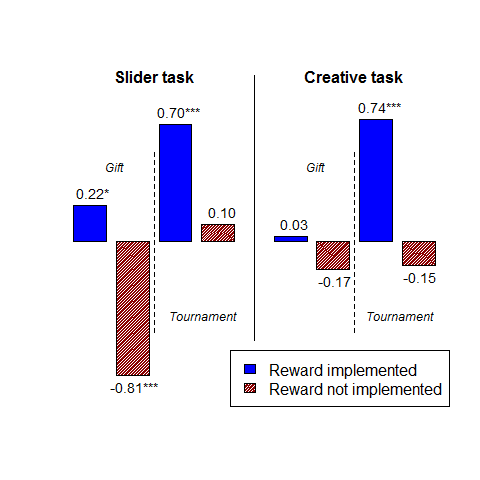
\includegraphics[width=0.75\textwidth]{Graphs/160308_Neg_Bonus_Dec.png}
\label{fig:Neg_Bonus_Dec}
	\begin{minipage}{0.8\textwidth}
	\footnotesize
	\vspace{5mm}
	{\it Note:} The dependent variable is standardized performance of agents in Period 2. The bars show the estimated regression coefficients of separate OLS regressions. Performance is measured as the number of correctly positioned sliders in the simple task and as the score achieved in the creative task. The regressions control for baseline performance in Period 1. The respective control group (slider or creative) serves as the reference category. Statistical significance: * p < 0.1, ** p < 0.05, *** p < 0.01. 
	\end{minipage}
\end{center}
\end{figure}

%-	Das sind 8 seprarate Regressionen, die immer die Kontrollgruppe enthält sowie entweder %die Agenten die von positiven oder negativen Bonusentscheidungen betroffen waren also:
%-	Gift positive Bonusentscheidung im Vergleich mit Kontrollgruppe Slider
%Gift negative Bonusentscheidung im Vergleich mit Kontrollgruppe Slider
%-	Turnier positive Bonusentscheidung im Vergleich mit Kontrollgruppe Slider
%Turnier negative Bonusentscheidung im Vergleich




\newpage
\begin{figure}[H]
\caption{Overview of Effect Sizes for All Gift Treatments}
\begin{center}
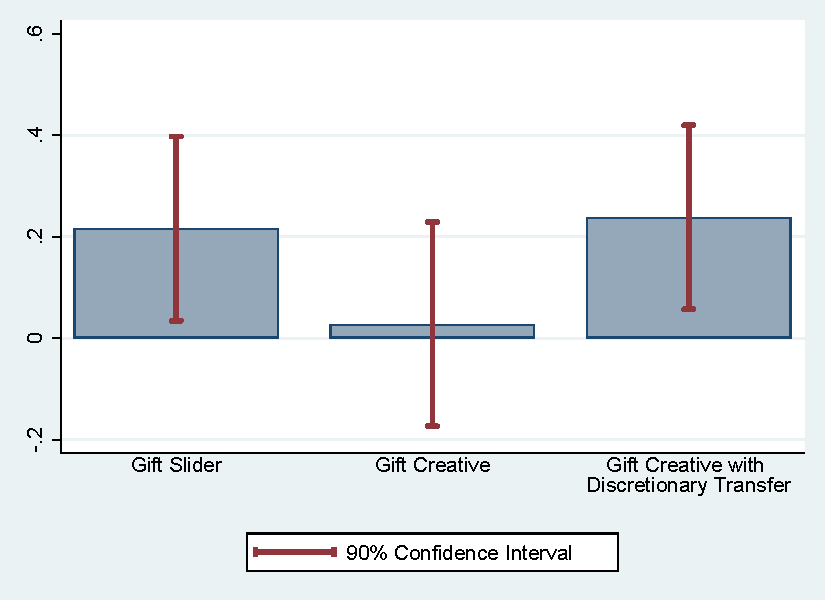
\includegraphics[width=0.75\textwidth]{Graphs/Figure5_new.pdf}
\label{fig:gift_treatments}
	\begin{minipage}{0.75\textwidth}
	\footnotesize
	\vspace{3mm}
	{\it Note:} The bars show the estimated regression coefficients of separate OLS regressions. Standardized performance (transfer) in Period 2 is the dependent variable. Performance is measured as the number of correctly positioned sliders in the simple  task,  as the score achieved in the creative task, and as the amount tranferred in the creative transfer treatments. The regression controls for baseline performance in Period 1. The respective control group serves as the reference category.
	\end{minipage}
\end{center}
\end{figure}



\newpage

\begin{figure}[H]
	\caption{Difference in Performance between Periods 3 and 1 by Treatment and Task}
	\label{fig:Bar_Chart_Round_1_3}
	\subfloat{\includegraphics[width=0.45\textwidth]{Graphs/Figure5a_paired_final3.pdf}}	
	\qquad
	\subfloat{\includegraphics[width=0.45\textwidth]{Graphs/Figure5b_paired_final3.pdf}}\\
	\begin{minipage}{0.9\textwidth}
	\footnotesize
	{\it Note:} The bars show the difference in mean performance between Period 3 and Period 1. The whiskers depict 90\% confidence intervals of paired t-tests. Note, this figure is on a bigger scale than Figure \ref{fig:Bar_Chart_Round_1_2} to improve readability.
	\end{minipage}
\end{figure}


\newpage
%\newpage
\input{Tables/Table_1_Creative_Answers_150114.tex}
%\newpage
\input{Tables/Table_3_Summary_Statistics_Appendix.tex}
%\newpage
\begin{table}[H]
\caption{Treatment Effects in Period 2}%
\begin{center}%
{\small\renewcommand{\arraystretch}{0.8}%
{\setlength{\tabcolsep}{7pt}
\begin{tabular}{lccc}
\hline\hline\noalign{\smallskip}
                    &\multicolumn{1}{c}{I}&\multicolumn{1}{c}{II}&\multicolumn{1}{c}{III}\\
\hline\noalign{\smallskip}
Tournament Treatment&       0.795***&       0.736***&       0.751***\\
                    &     (0.173)   &     (0.143)   &     (0.143)  \\[4mm]
Tournament x Slider-Task&       0.166   &      -0.058   &      -0.060     \\
                    &     (0.178)   &     (0.166)   &     (0.168)    \\[4mm]
Gift Treatment      &      -0.019   &       0.026   &      -0.006   \\
                    &     (0.143)   &     (0.099)   &     (0.103)    \\[4mm]
Gift x Slider-Task  &       0.375** &       0.209*  &       0.206*   \\
                    &     (0.170)   &     (0.109)   &     (0.112)    \\[4mm]
Baseline            &               &       0.657***&       0.638***\\
                    &               &     (0.076)   &     (0.076)      \\[4mm]
Baseline x Slider-Task&               &       0.002   &       0.028    \\
                    &               &     (0.094)   &     (0.094)     \\[4mm]
Intercept           &      -0.000   &      -0.000   &       0.874    \\
                    &     (0.093)   &     (0.062)   &     (0.595)    \\[2mm]
\hline
Controls           &      NO   &      NO   &       YES    \\
\hline
Observations        &         348   &         348   &         348     \\
$R^2$               &       0.146   &       0.546   &       0.564      \\
\hline\hline\noalign{\medskip}
\end{tabular}}
\begin{minipage}{0.8\textwidth}
\footnotesize
{\it Note:} This table reports the estimated OLS coefficients from Equation \ref{eq:reg}. The dependent variable is the standardized performance in Period 2 and refers to the number of sliders moved in the simple task and the creativity score in the creative task. The coefficient on the \textit{Tournament} (\textit{Gift}) treatment represents the impact of the \textit{Tournament} (\textit{Gift}) on the creative task. The interaction effect between the respective treatment and the slider task documents whether the response to the \textit{Tournament} (\textit{Gift}) differs between the creative and the simple task. The impact of the tournament (\textit{Gift}) on the simple task is equal to the sum of the coefficient on the treatment and its interaction effect.\\
The estimation includes all agents from the Control Group as well as agents from treatment groups where the principal decided to institute the tournament/gift. Agents with negative reward decisions are not part of this analysis. Additional control variables are age, age squared, sex, location, field of study as well as a set of time fixed  effects (semester period, semester break, exam period). Heteroscedastic-robust standard errors are reported in parentheses. Significance levels are denoted as follows: * $p < 0.1$, ** $p < 0.05$, *** $p < 0.01$. 
\end{minipage}}
\end{center}
\label{tab:EQ_Pooled_Results}
\end{table}

\newpage
\begin{table}[H]
\caption{Effects Creative Transfer }%
\begin{center}%
{\small\renewcommand{\arraystretch}{0.8}%
{\setlength{\tabcolsep}{7pt}
\begin{tabular}{lcc}
\hline\hline\noalign{\smallskip}
    & \multicolumn{2}{c}{\textbf{Amount Transferred}}\\
\hline\noalign{\smallskip}
Gift	&	0.224**	&	0.264**  \\
	&	(0.103)	&	(0.126)	\\[4mm]
Baseline Transfer	&	0.653***	&	0.653***	\\
	&	(0.063)	&	(0.061)	\\[4mm]
Intercept	&	-0.000	&	-0.677	\\
	&	(0.077)	&	(0.851)	\\[2mm]
\hline
Controls           &   No   &       YES   \\
\hline
Observations	 &         139   &         139   \\ 
$R^2$               &       0.515   &       0.540 \\
\hline\hline\noalign{\medskip}
\end{tabular}}
\begin{minipage}{0.8\textwidth}
\footnotesize
{\it Note:} This table reports the estimated OLS coefficients from Equation \ref{eq:reg}. The dependent variable is the standardized amount transferred in Period 2. Amount transferred refers to the treatment in which agents work on the creative task, are informed about the number of points that they generated with their answers and can then decide how many of those points to transfer to their principal. The coefficient on the \textit{Tournament} (\textit{Gift}) treatment represents the impact of the \textit{Tournament} (\textit{Gift}) on the creative task. The interaction effect between the respective treatment and the slider task documents whether the response to the \textit{Tournament} (\textit{Gift}) differs between the creative and the simple task. The impact of the tournament (\textit{Gift}) on the simple task is equal to the sum of the coefficient on the treatment and its interaction effect.\\
The estimation includes all agents from the Control Group as well as agents from treatment groups where the principal decided to institute the tournament/gift. Agents with negative reward decisions are not part of this analysis. Additional control variables are age, age squared, sex, location, field of study as well as a set of time fixed  effects (semester period, semester break, exam period). Heteroscedastic-robust standard errors are reported in parentheses. Significance levels are denoted as follows: * $p < 0.1$, ** $p < 0.05$, *** $p < 0.01$. 
\end{minipage}}
\end{center}
\label{tab:Feedback}
\end{table}
%\newpage
\begin{landscape}
\begin{table}
\caption{Dimensions of Creativity: Treatment Effects on Standardized Performance in Period 2}
\begin{center}%
{\small\renewcommand{\arraystretch}{0.9}%
\begin{tabular}{lcccccccc}
\hline\hline\noalign{\smallskip}
 &     \multicolumn{7}{c}{\bf Creative Task}  &\\
&    \it Score &  \it Validity  &  \it Flexibility & \it Originality & \it Flexibility Rate  & \it Originality Rate  & \it Top Answers & \it Invalid Uses   \\
&          I       &      II         &       III         &       IV          &     V     & VI & VII & VIII      \\
\hline\noalign{\smallskip}		

Tournament & 0.753*** & 0.813*** & 0.607*** & 0.726*** & -0.035 & 0.106* & 0.199** & 0.286\\
&(0.162) &(0.171) & (0.151) & (0.180) & (0.045) & (0.062) & (0.087) & (0.208)\\[4mm]
Gift & -0.059 & -0.027 & -0.041 & -0.143 & 0.014 & -0.083 & 0.011 & -0.178\\
&(0.124) &(0.131) & (0.120) & (0.150) & (0.048) & (0.068) & (0.087) & (0.187)\\[4mm]
Period 1 & 0.614*** & 0.581*** & 0.598*** & 0.552*** & 0.058 & 0.081 & 0.197*** & 0.262***\\
&(0.077) &(0.078) & (0.071) & (0.087) & (0.063) & (0.089) & (0.061) & (0.065)\\
\noalign{\smallskip}\hline\noalign{\smallskip}
Intercept         	&		YES		&		YES		&		       YES   		&		 YES 		&		 YES 		&		 YES 		&			 YES 	&		 YES 		\\	\hline
Controls           	&		YES		&		YES		&		       YES   		&		 YES 		&		 YES 		&		 YES 		&			 YES 	&		 YES 		\\	\hline
Observations 	&		172		&		172		&		172		&		172		&		152		&		152		&		172		&		172		\\	
$R^2$        	&		0.500		&		0.474		&		0.526		&		0.389		&		0.068		&		0.117		&		0.179		&		0.190		\\	
\hline\hline\noalign{\medskip}
\end{tabular}}
\begin{minipage}{1.25\textwidth}
\footnotesize
{\it Note:} This table reports OLS estimates of Equation \ref{eq:reg}, where we regress (standardized) performance in Period 2 on baseline performance and treatment dummies. Column I reports results on the aggregated creativity score. Columns II, III and V report the results on the different standardized sub-dimensions of the creativity score.  Column IV and VI displays treatment effects on the (unstandardized) flexibility and originality rate. The flexibility (originality) rate equals achieved flexibility (originality) points divided by the total number of subject's valid answers (subjects with zero valid answers were dropped in these columns). Column VII reports results for an assesment of the best creative answers from an evaluator blind to the treatments. Column VIII report results for invalid uses.\\
The estimation includes all agents from the Control Group as well as agents from treatment groups where the principal decided to institute the tournament/gift. Agents with negative reward decisions are not part of this analysis. Additional control variables are age, age squared, sex, location, field of study as well as a set of time fixed  effects (semester period, semester break, exam period). Heteroscedastic-robust standard errors are reported in parentheses. Significance levels are denoted as follows: * $p < 0.1$, ** $p < 0.05$, *** $p < 0.01$.
%\textsuperscript{1} The flexibility (originality) rate equals achieved flexibility (originality) points divided by the number of subject's valid answers. The sample size is reduced to 215 observations because we cannot calculate the flexibility or originality rate (or it's baseline) for individuals who do not provide any answers in either period 1 or period 2.
\end{minipage}
\label{tab:EQ1_Main_Regression_Creative_Task}
\end{center}
\end{table}
\end{landscape}

\clearpage
%\newpage
%\input{Tables/Table_8_Summary_Statistics_EKE_KEK_130322.tex}
\clearpage
\newpage





\setcounter{section}{0}
\renewcommand*{\theHsection}{chX.\the\value{section}}
\section*{Appendix}
\subsection*{Translated Instructions (Original in German)} \label{instructions}
\input{Instructions_final.tex} 
%\section{Mixed Task Treatments}
\label{mixed}

To shed light into whether the positive post-treatment effect of winning the tournament 
is task-specific or stems from a general mood effect that should raise performance in any subsequent task, we conducted two 
supplementary tournament treatments. In these supplementary treatments, subjects were asked to 
work on both the routine and the creative task in alternating orders (either 
slider (Period 1) - creative (Period 2) - slider (Period 3) (\textit{SCS}) or 
creative (Period 1) - slider (Period 2) - creative (Period 3) (\textit{CSC}). 
Identical to the main \textit{Tournament} treatments, 
agents received fixed wages in Periods 1 and 3, and the principal could 
implement a tournament in Period 2. In total, 55 subjects participated in the 
\textit{ Slider-Creative-Slider (SCS)} treatment, and 46 subjects 
 in the \textit{ Creative-Slider-Creative (CSC)} treatment. 
The right-hand  columns of Table \ref{tab:Summary_Statistics} show 
summary statistics for these observations. There are no significant differences in 
baseline performance between these two  supplementary tournament treatments 
and the respective control groups. For this comparison, and for analyzing treatment effects below, 
we use the creative task control group as a benchmark for 
baseline performance and  Period 3 performance in \textit{CSC}, 
and the slider task control group to assess 
performance in Periods 1 and 3 in \textit{SCS}. Note that we did not include 
additional control groups with varying tasks but without the tournament. 
We therefore cannot control for changes in Period 3 performance 
that are caused by the change in the tasks per se, rendering our findings below suggestive 
rather than conclusive. 
Table \ref{tab:reg_spillover} presents the results on Period 3 performance. 
The results are split up by treatment and task.\\


%\begin{landscape}
\begin{table}[!htbp]
\caption{\label{tab:reg_spillover} Post-treatment  Effects of the Tournament in Period 3 by Task}%
\begin{center}%
{\small\renewcommand{\arraystretch}{0.7}%
\begin{tabular}{lcccccccc}
\hline\hline\noalign{\smallskip}
  & & & & & \multicolumn{4}{c}{\bf Mixed Tasks} \\
 	&   \multicolumn{2}{c}{\bf Slider Task} & \multicolumn{2}{c}{\bf Creative Task} &\multicolumn{2}{c}{\bf Slider-Creative-Slider} & \multicolumn{2}{c}{\bf Creative-Slider-Creative} \\
 & & & & & \multicolumn{2}{c}{\bf (SCS)} & \multicolumn{2}{c}{\bf (CSC)}\\	
 & I & II & III & IV & V & VI & VII & VIII \\
\hline\noalign{\smallskip}
Tournament & 0.245* &  & 0.340*** &  & 0.111 &  & 0.055 &  \\
 & (0.137) &  & (0.126) &  &  (0.109)&  & (0.121) &  \\[2mm]
Tournament Winner &  & 0.534*** &  & 0.449*** &  & 0.064 &  & 0.091 \\
 &  & (0.180) &  & (0.170) &  & (0.122) &  & (0.146) \\[2mm]
Tournament Loser &  & -0.030 &  & 0.236* &  & 0.158 &  & 0.007 \\
 &  & (0.146) &  & (0.134) &  & (0.142) &  & (0.132) \\[2mm]
Standardized Performance & 0.888*** & 0.848*** & 0.693*** & 0.670*** & 0.888*** & 0.891*** & 0.648*** & 0.648*** \\
in Period 1 & (0.060) & (0.063) & (0.080) & (0.086) & (0.052) & (0.053) & (0.089) & (0.090) \\ [2mm]
Intercept & 0.000 & 0.000 & 0.000 & 0.000 & 0.000 & 0.000 & 0.000 & 0.000 \\
 & (0.073) & (0.073) & (0.093) & (0.094) & (0.073) & (0.073) & (0.094) & (0.094) \\[2mm]
\hline\noalign{\smallskip}
Observations & 116 & 116 & 116 & 116 & 115 & 115 & 102 & 102 \\
 R-squared & 0.679 & 0.708 & 0.529 & 0.535 & 0.734 & 0.735 & 0.503 & 0.504 \\
\hline\hline
\end{tabular}}
\begin{minipage}{1.2\textwidth}
\footnotesize
\vspace{5mm}
{\it Note:} This table reports OLS estimates of standardized performances in Period 3. Performance is measured as the number of correctly positioned sliders in the simple task and as the score in the creative task, respectively.\\ 
The estimation includes all agents from the Control Group as well as agents from treatment groups where the principal decided to institute the tournament as well as agents from the supplementary treatments SCS and CSC. Agents with negative reward decisions are not part of this analysis. Heteroscedastic-robust standard errors are reported in parentheses. Significance levels are denoted as follows: * $p < 0.1$, ** $p < 0.05$, *** $p < 0.01$.
\end{minipage}
\end{center}
\end{table}
\end{landscape}

Columns I and II report results from the slider task (overall and split up by winners and losers). 
Columns III and IV do the same for the creative task. Analogously, Period 3 treatment effects on the 
the mixed tasks \textit{SCS} and \textit{CSC} are depicted in columns V-VIII. 
Each regression controls for baseline performance and compares effects to the respective control group.
We find no evidence for positive spillover effects -- neither overall nor for winners or losers separately. 
The treatment effects in the mixed tasks treatments, \textit{SCS} and \textit{CSC} (Columns V-VIII) are positive 
but small and statistically insignificant. Hence,  winning  a tournament or receiving positive feedback 
may lead to higher subsequent performance, but we have suggestive evidence that such an increase is limited to the task at hand. Possible 
mechanisms are increased task-specific self-confidence or intrinsic motivation. Our data does not lend
support for more general and task-unspecific effects on intrinsic motivation, such as mood effects. 
%\section{Feedback Treatment}
\label{feedback}

%Tournaments affect behavior via two different channels: 1) a concern for a good relative standing and 
%2) the monetary incentive (the tournament prize). For policy, it is important to understand how much of the tournament effect 
%is driven by the (costly) prize and how much is driven by (cheap) relative performance information. 
% To disentangle these two channels, we conducted a \textit{Feedback} treatment that conveyed
% the same information about relative rank than the \textit{Tournament} treatment 
%but without monetary consequences. In the \textit{Feedback} treatment, the principal had to 
%decide before the start of period 2 whether or not  relative rank information would be provided 
%to her agents at the end of period 2. The provision of relative performance feedback was 
%costless to the principal and payoffs in this treatment were identical to those in the 
%control group in all three rounds. In case the principals opted for feedback provision, 
%agents were informed at the beginning of period 2 that they would learn at the end of period 2 
%whether or not they belonged to the best 50\% of their group. 
%We observe 56 agents with positive reward decisions in the Slider task and 68 agents 
%with positive reward decisions in the Creative task in this treatment.



%\section{Number of Breaks}
\label{breaks}


%\newpage
\input{Tables/Table_6_Breaks_150108.tex}
\clearpage
\subsection*{Webappendix} \label{instructions}
%\newpage
\begin{landscape}
{\small
\begin{table}\caption{ Overview of Payoffs by Treatment, Role, and Period}
\smallskip
\begin{tabular}[H]{|l|cc|cc|cc|}\hline\hline
\multicolumn{7}{|c|}{\textbf{Payments in Taler}}\\\hline
& \multicolumn{2}{c|}{Control} & \multicolumn{2}{c|}{Gift} & \multicolumn{2}{c|}{Tournament}\\\hline
& Principal & Agent & Principal & Agent & Principal & Agent\\\hline
Period 1 - Fixed Wage & 300 & 300 & 300 & 300 & 300 & 300\\\hline
Period 2 &  &  &  &  &  &  \\
\hspace{0.4cm} Fixed Wage & 100 & 600 & 300 & 300 & 300 & 300 \\
\hspace{0.4cm} Reward Costs(-)/Benefits(+) & - & - & -200 & +300 & -200 & \hspace{0.2cm} +0/600$^{a}$ \\\cdashline{1-7}
\hspace{0.4cm} Total (Expected) Payoff & 100 & 600 & 100 & 600 & 100 & \hspace{0.3cm} 600$^{b}$  \\ \hline
Period 3 - Fixed Wage & 300 & 300 & 300 & 300 & 300 & 300 \\\hline\hline
\end{tabular}


\begin{minipage}{0.84\textwidth}
\footnotesize
\vspace{5mm}
\textit{Note}: 
$^{a}$ Tournament winners (best 50\%) receive a bonus of 600 Taler and tournament losers (worst 50\%) receive nothing. \\
$^{b}$ Assuming risk neutrality and a 50\% chance of winning, a subject's expected earnings in the tournament treatment at the beginning of the second period as well as average earnings at the end of the second period are 600 Taler.\\
The experimental currency unit ``Taler'' was converted into Euros at an exchange rate of 100 Taler = 1 Euro.
   \end{minipage}

\vspace{5mm}
\begin{tabular}[H]{|l|l|}\hline\hline
\multicolumn{2}{|l|}{\textbf{Variable Payments (in Taler):}}\\\hline
\textbf{Principal:} &\\
Per Slider & 5\\\hline
Per Valid Answer & 5\\
Per Category & 5\\
Per Original Answer & 5\\
Per Very Original Answer & 10\\\hline
\textbf{Agent:} &\\
Per Time-out & 5\\\hline\hline
\end{tabular}
\label{tab:Pay_Off_Design}
\end{table}}
 \end{landscape}

\newpage
\input{Tables/WebAppendix/Table_3_Summary_Statistics_Webappendix}
\newpage
\begin{landscape}
\begin{table}\caption{Sensitivity Analyses}
\begin{center}%
{\small\renewcommand{\arraystretch}{0.8}%
{\setlength{\tabcolsep}{7pt}
\begin{tabular}{l*{7}{c}}
\toprule
                    &\multicolumn{1}{c}{Score}&\multicolumn{1}{c}{Validity}&\multicolumn{1}{c}{Flexiblity}&\multicolumn{1}{c}{Originality 10\%}&\multicolumn{1}{c}{Originality 5\%}&\multicolumn{1}{c}{Originality 1\%} & \multicolumn{1}{c}{Invalid Uses}\\
\midrule
Gift                		&	0.026	&		      0.054         		&		      0.055         		&		      -0.101         		&		     -0.075         		&		       0.237			&		      -0.112         			\\
                    		&	(0.121)	&		      (0.125)         		&		      (0.116)         		&		     (0.141)         		&		     (0.143)         		&		      (0.190)	&		     (0.181)         			\\\addlinespace
Tournament             		&	0.736***	&		       0.789***		&		       0.589***		&		       0.683***		&		       0.672***		&		       0.747**	&		       0.294         			\\
                    		&	(0.160)	&		      (0.168)         		&		      (0.146)         		&		      (0.190)         		&		      (0.193)         		&		      (0.194)		&		      (0.216)         			\\\addlinespace
Baseline		&	0.657	&		       0.628***		&		       0.628***		&		       0.512***		&		       0.564***		&		       0.557**		&		       0.255***			\\
Performance		&	(0.076)	&		      (0.099)         		&		      (0.092)         		&		      (0.083)         		&		      (0.090)         		&		      (0.117)		&		      (0.071)         			\\
\midrule																
Intercept 	&	  Yes 	&	  Yes 	&	  Yes 	&	  Yes 	&	  Yes 	&	  Yes	&	 Yes 		 \\\midrule
R$^2$ 	&	0.473	&	0.433	&	0.5	&	0.309	&	0.311	&	0.257	&	0.128		\\
Observations        	&	172	&	172	&	172	&	171	&	171	&	171	&	172		\\
\bottomrule
\end{tabular}}
\begin{minipage}{0.75\linewidth}
\footnotesize
\vspace{5mm}
{\it Note:} This table reports OLS estimates of Equation \ref{eq:reg}, where we regress standardized performance in Period 2 on baseline performance and treatment dummies. Column I reports results on invalid uses. Columns II to VI report the results on the different sub-dimensions of the creativity score. Column IV to VI report robustness for the calculation of the originality score 
(given exactly point for each \textit{original} answer given by less than 10\%, 5\% or 1\% of agents).\\
The estimation includes all agents from the Control Group as well as agents from treatment groups where the principal decided to institute the tournament/gift. Agents with negative reward decisions are not part of this analysis. Heteroscedastic-robust standard errors are reported in parentheses. Significance levels are denoted as follows: * $p < 0.1$, ** $p < 0.05$, *** $p < 0.01$.
\end{minipage}}
\label{tab:Summary_Statistics}
\end{center}
\end{table}
%}
\end{landscape}
\newpage
\input{Tables/WebAppendix/Table_Ex-Post_Short.tex}
\newpage
\input{Tables/WebAppendix/Table_Feedback.tex}
\newpage
\begin{landscape}
\begin{table}[!htbp]
\caption{\label{tab:reg_spillover} Post-treatment  Effects of the Tournament in Period 3 by Task}%
\begin{center}%
{\small\renewcommand{\arraystretch}{0.7}%
\begin{tabular}{lcccccccc}
\hline\hline\noalign{\smallskip}
  & & & & & \multicolumn{4}{c}{\bf Mixed Tasks} \\
 	&   \multicolumn{2}{c}{\bf Slider Task} & \multicolumn{2}{c}{\bf Creative Task} &\multicolumn{2}{c}{\bf Slider-Creative-Slider} & \multicolumn{2}{c}{\bf Creative-Slider-Creative} \\
 & & & & & \multicolumn{2}{c}{\bf (SCS)} & \multicolumn{2}{c}{\bf (CSC)}\\	
 & I & II & III & IV & V & VI & VII & VIII \\
\hline\noalign{\smallskip}
Tournament & 0.245* &  & 0.340*** &  & 0.111 &  & 0.055 &  \\
 & (0.137) &  & (0.126) &  &  (0.109)&  & (0.121) &  \\[2mm]
Tournament Winner &  & 0.534*** &  & 0.449*** &  & 0.064 &  & 0.091 \\
 &  & (0.180) &  & (0.170) &  & (0.122) &  & (0.146) \\[2mm]
Tournament Loser &  & -0.030 &  & 0.236* &  & 0.158 &  & 0.007 \\
 &  & (0.146) &  & (0.134) &  & (0.142) &  & (0.132) \\[2mm]
Standardized Performance & 0.888*** & 0.848*** & 0.693*** & 0.670*** & 0.888*** & 0.891*** & 0.648*** & 0.648*** \\
in Period 1 & (0.060) & (0.063) & (0.080) & (0.086) & (0.052) & (0.053) & (0.089) & (0.090) \\ [2mm]
Intercept & 0.000 & 0.000 & 0.000 & 0.000 & 0.000 & 0.000 & 0.000 & 0.000 \\
 & (0.073) & (0.073) & (0.093) & (0.094) & (0.073) & (0.073) & (0.094) & (0.094) \\[2mm]
\hline\noalign{\smallskip}
Observations & 116 & 116 & 116 & 116 & 115 & 115 & 102 & 102 \\
 R-squared & 0.679 & 0.708 & 0.529 & 0.535 & 0.734 & 0.735 & 0.503 & 0.504 \\
\hline\hline
\end{tabular}}
\begin{minipage}{1.2\textwidth}
\footnotesize
\vspace{5mm}
{\it Note:} This table reports OLS estimates of standardized performances in Period 3. Performance is measured as the number of correctly positioned sliders in the simple task and as the score in the creative task, respectively.\\ 
The estimation includes all agents from the Control Group as well as agents from treatment groups where the principal decided to institute the tournament as well as agents from the supplementary treatments SCS and CSC. Agents with negative reward decisions are not part of this analysis. Heteroscedastic-robust standard errors are reported in parentheses. Significance levels are denoted as follows: * $p < 0.1$, ** $p < 0.05$, *** $p < 0.01$.
\end{minipage}
\end{center}
\end{table}
\end{landscape}
\newpage

%\begin{landscape}
\begin{table}[H]%
\caption{Treatment Effects in Period 2 -- Controlling for Number of Breaks Taken}
\begin{center}%
{\small\renewcommand{\arraystretch}{0.7}%
\begin{tabular}{lcc}
\hline\hline\noalign{\smallskip}
            &      Slider Task   &    Creative Task   \\
						&          I         &       II           \\
\hline\noalign{\smallskip}
Gift Treatment&       0.019   &      -0.056   \\
            &     (0.056)   &     (0.110)   \\[2mm]
Tournament Treatment&       0.156** &       0.269** \\
            &     (0.064)   &     (0.125)   \\[2mm]
%Feedback Treatment&       0.086   &      -0.017   \\
%            &     (0.065)   &     (0.101)   \\[2mm]
1 to 3 Breaks (Period 1)    &      -0.076*  &      -0.188  \\
            &     (0.117)   &     (0.169)   \\[2mm]
4 to 7 Breaks (Period 1)    &      -0.362*&      -0.122   \\
            &     (0.186)   &     (0.168)   \\[2mm]
8 or more Breaks (Period 1) &      -0.630**&      -0.573***\\
            &     (0.250)   &     (0.196)   \\[2mm]
Difference between the      &      -0.734***&      -0.204***\\
 Breaks in Periods 2 and 1  &     (0.146)   &     (0.061)   \\[2mm]
1 to 3 Breaks (Period 1)    &       0.530***  &      -0.031   \\
   $\times$  Break Difference           &     (0.149)   &     (0.071)   \\[2mm]
4 to 7 Breaks (Period 1)    &       0.461***   &       0.030   \\
   $\times$  Break Difference           &     (0.147)   &     (0.078)   \\[2mm]
8 or more Breaks (Period 1) &       0.414***   &      -0.082   \\
   $\times$  Break Difference           &     (0.146)   &     (0.080)   \\[2mm]
Standardized&       0.767***&       0.721***\\
Performance in Period 1          &     (0.095)   &     (0.077)   \\[2mm]
Intercept   &       0.141  &       0.275* \\
            &     (0.132)   &     (0.163)   \\[2mm]
\hline\noalign{\smallskip}
Observations&         176   &         172   \\
$R^2$       &       0.915   &       0.677   \\
\hline\hline\noalign{\medskip}
\end{tabular}}
\begin{minipage}{0.70\textwidth}
\footnotesize
{\it Note:} In order to create a more realistic work environment  in which agents face opportunity costs of working, we implemented a time-out button (see Section \ref{sec:groups}) which was displayed at the bottom of the screen during all working periods. Each time agents clicked the time-out button, the computer screen was locked for 20 seconds, prohibiting the entry of creative ideas or the movement of sliders, and 5 Taler were added to the agent's payoff.\\ 
This table reports OLS coefficient estimates from our main model specification (Equation \ref{eq:reg},  with the number of breaks in period 1, the change in breaks between periods 1 and 2, as well as interactions between the two as additional controls. Standardized performance in period 2 is the dependent variable. Performance is measured as the number of correctly positioned sliders in the simple task and as the score in the unusal uses, creative task, respectively.\\
The estimation includes all agents from the Control Group as well as agents from treatment groups where the principal decided to institute the tournament/gift. Agents with negative reward decisions are not part of this analysis. Heteroscedasticity-robust standard errors including a degree of freedom correction are reported in parentheses. Significance levels are denoted as follows: * $p < 0.1$, ** $p < 0.05$, *** $p < 0.01$. \end{minipage}
\end{center}
\label{tab:EQ_Breaks_Results}
\end{table}
%\end{landscape}



\end{document}

